% ============================================================
%  R. Nielsen, "Philosophie og Mathematik. En propædeutisk Afhandling."
%  "Philosophy and Mathematics. A Propaedeutic Treatise."
%  Kjøbenhavn: Forlagt af den Gyldendalske Boghandling (F. Hegel);
%  Thieles Bogtrykkeri, 1857.
%  TRANSLATION (English) — from the verified Danish transcription.tex.
%
%  Method: prose-only translation. Every equation, array, tikzpicture
%  block (with its % FIGURE comment), point/label token, and % flag
%  print-oddity note is carried over VERBATIM from transcription.tex;
%  only natural-language prose (body sentences, footnote prose, heading
%  titles, caption words) is translated. See TRANSLATION-HANDOFF.md.
%
%  Register: scholarly, moderately literal, preserving Nielsen's
%  speculative/Hegelian flavour wrapped around real analysis.
%
%  STATUS: IN PROGRESS. Done: front matter + Section I (printed pp.3--18).
%        Resume at Section II ("The Problem of Infinity", printed p.19).
% ============================================================
\documentclass[12pt]{book}
\usepackage[utf8]{inputenc}
\usepackage[T1]{fontenc}
\usepackage[english]{babel}
\usepackage[protrusion=true,expansion=true]{microtype}
\usepackage[margin=1.4in]{geometry}
\usepackage{setspace}
\usepackage{amsmath}
\usepackage{graphicx}
\usepackage{tikz}
\usetikzlibrary{calc,intersections,arrows.meta}
\usepackage{libertinus}
\usepackage{libertinust1math}
\usepackage{textalpha}   % polytonic Greek typed directly
\usepackage{fancyhdr}
\usepackage[colorlinks=true,linkcolor=black,urlcolor=black,
  pdftitle={Philosophy and Mathematics},
  pdfauthor={Rasmus Nielsen}]{hyperref}
\setlength{\headheight}{15pt}
\pagestyle{fancy}
\fancyhf{}
\fancyhead[LE,RO]{\thepage}
\fancyhead[RE]{\textit{Philosophy and Mathematics}}
\fancyhead[LO]{\textit{\leftmark}}
\setlength{\parindent}{1.5em}
\setlength{\parskip}{0pt}
\onehalfspacing

\begin{document}

% ============================================================
% TITLE PAGE — PDF 6 (printed p.1)
% ============================================================
\begin{titlepage}
\centering
\vspace*{2cm}
{\Huge\bfseries Philosophy and Mathematics.\par}
\vspace{1.2cm}
\rule{4cm}{0.4pt}\par
\vspace{1.2cm}
{\LARGE A Propaedeutic Treatise\par}
\vspace{0.5cm}
{\large by\par}
\vspace{0.8cm}
{\LARGE\bfseries R.\ Nielsen,\par}
\vspace{0.2cm}
{\normalsize Professor of Philosophy.\par}
\vspace{2.4cm}
\rule{4cm}{0.4pt}\par
\vspace{1.6cm}
{\large\bfseries Kjøbenhavn.\par}
\vspace{0.4cm}
{\normalsize Forlagt af den Gyldendalske Boghandling (F.\ Hegel).\par}
\vspace{0.3cm}
{\small\emph{Thieles Bogtrykkeri.}\par}
\vspace{0.6cm}
{\large 1857.\par}
\end{titlepage}

\frontmatter
\tableofcontents
\mainmatter

% ============================================================
% BODY BEGINS — printed p.3 (PDF 8)
% ============================================================

% ---- printed p.3 (PDF 8): opening statement (stands alone on the page) ----
\noindent The author of the present treatise, who neither is nor wishes to be
a mathematician, has found in philosophy, the general theory of science, an
incitement to learn the language of mathematics as well, and, with respect to
its leading fundamental concepts, so far as possible, to enter into its way of
thinking.

% ---- printed p.4 (PDF 9): "Rettelse." (errata). Original page (letterspaced
%      heading) reads only:
%        S. 25, Linie 9: Tilnærmelse til et Uopnaaeligt; læs: Tilnærmelse til
%        et Opnaaeligt.
%      Per repo convention the errata page is NOT reproduced as body text;
%      the correction is APPLIED where p.25 is translated (Section II): the
%      text there must read "an approach toward an Attainable".

% ============================================================
% ---- printed p.5 (PDF 10) ----
\begin{center}
  {\large\bfseries I.}\par\vspace{4pt}
  {\Large\bfseries Mathematical Functions.}\par\vspace{4pt}
  \rule{2.5cm}{0.4pt}
\end{center}
\phantomsection
\addcontentsline{toc}{section}{\texorpdfstring{I.\quad Mathematical Functions}{I. Mathematical Functions}}
\markboth{Mathematical Functions}{Mathematical Functions}

\noindent The word ``function'' occurs in a very wide sense. Wherever there can
be talk of acting, suffering, doing, function denotes a particular law-governed
activity. It is said of an official\footnote{With categorical emphasis
Chamberlain Norden in ``Gamle Minder'' stresses his ``term of function.''}, that
he is in function; one speaks of the function of the eye, of the function of a
nerve, and so forth.

On the domain of pure magnitudes there can, as regards these, just as little be
talk of real doing as of real suffering: an $a$ cannot act, a $b$ cannot suffer,
an $x$ cannot function in the likeness either of an official or of a nerve.

Since nevertheless the designation ``function'' is not only retained, but even
held fast as a concept in mathematics, one must be able, in the mathematical
application, to point out something corresponding to the fundamental meaning.

To be sure, pure magnitudes cannot exert real activity, but by being placed in
different connections they can nevertheless essentially alter their mutual
relations. A magnitude can, so to speak, be appointed to different offices; it
can, as an addend $(a+x)$, as a factor $(ax)$, as an exponent of a power
$(a^{x},\ x^{a})$, as a logarithm, and so forth, acquire a
% ---- printed p.6 (PDF 11) ----
very different influence, and to that extent appear in different functions.

Here, however, is another side of the concept, which must be brought out
especially in the theory of magnitude. One speaks not merely of functioning, of
being in function; one speaks also of that which is brought about by the
functioning activity. Outside mathematics one thinks, in connection with
function, chiefly of the activity, in mathematics chiefly of the result;
outside mathematics the point is to be in function at something, within
mathematics to be a function of something. The law-bound relation between a
dependent and an independent shows itself, however, on both sides.

``If a magnitude $y$ depends, according to a certain law, on other magnitudes
$x$, $z$, $t$, $u\ldots$, so that every value of $y$ is determined by the values
arbitrarily assigned to $x$, $z$, $t$, $u\ldots$, then $y$ is said to be a
function of these magnitudes, all regarded as variable, $y$ dependent, the
others independent. This is commonly denoted: $y = f(x,z,t,u\ldots)$''\footnote{C.\
Ramus. Algebra og Functionslære. Kjøbenhavn 1840, S.\ 14.}.

According to this mathematical determination of the concept, changes will thus
proceed from the independents and exert their lawful influence upon the
dependent. In order to recall the likeness between non-mathematical and
mathematical functions, one might indeed regard the independents $x$, $z$, $t$,
$u\ldots$ as the functioning ones, the agents, that cause the changes in the
suffering $y$. But since the conception is figurative, one likewise sees why
$x$, $z$, $t$, $u\ldots$ are not said to be in function with respect to $y$,
whereas $y$ is expressly said to be a function of $x$, $z$, $t$, $u\ldots$

In the function, then, the magnitudes are variable; but magnitudes can of course
also be invariable. That every magnitude must be equal to itself, and that every
magnitude can, by increase or decrease, at every moment become
% ---- printed p.7 (PDF 12) ----
unequal to itself, is a contradiction that is resolved in the concept of
function. In and for itself no magnitude is either invariable or variable, for
no magnitude is anything alone in and for itself. Whether the particular
magnitude, on the other hand, in its relation to other magnitudes, is to play
the role of the invariable or of the variable, and, within variability, again
that of the dependent or of the independent, is determined by the function, and
in turn determines the function.

If the concept function is now, in the first place, determined by the concept of
dependence, then it depends again on determining the mode of dependence, that is
to say: on pointing out the law.

In the mathematical presentation of the different functions there shows itself a
scale of case, rule, and law, which must become an object of philosophy's
attention.
\[
\begin{aligned}
&\text{That }\ 2(3+4) = 2\cdot 3 + 2\cdot 4 = 6+8 = 2\cdot 7 = 14,\\
&\text{that }\ (3\cdot 4)^{2} = 12^{2} = 3^{2}\cdot 4^{2} = 9\cdot 16 = 144,\\
&\text{that }\ 2^{3}\cdot 2^{4} = (2\cdot 2\cdot 2)\cdot(2\cdot 2\cdot 2\cdot 2)
      = 2^{3+4} = 2^{7},
\end{aligned}
\]
can be experienced by trial, and seen by comparison. In this way one can test
various cases and abstract a rule from them. But, however important the rule may
be for practical use, it is nevertheless not, like the law, a necessary
expression of the essence of the matter.

In order to obtain a rule as comprehensive as possible, one must test as many
cases as possible; but even if one tested cases by the thousand without meeting
a single exception, the rule could not thereby be raised to a law.

The rule expresses only \emph{that a relation is}, not that it necessarily must
be; but the law holds as law in virtue of the concept. That, when the law is to
be known, it does not depend on the number of cases, but on \emph{the essence of
the matter}, and hence on insight, can be seen from the following example.

That $\frac{1}{1-x} = 1 + x + x^{2} + \ldots$ will yield an infinite series is
proved not by continuing the division to infinity,
% ---- printed p.8 (PDF 13) ----
but by understanding what the division, on the given presupposition,
necessarily brings with it.

How easily a series of cases falling under a rule can deceive, when one would
from this infer a law, is well known. One seeks, for example, a law for the
prime numbers, and finds: $2^{3}-1 = 7$, $2^{5}-1 = 31$, $2^{7}-1 = 127$, all
prime numbers. But if one now, from these three cases, would draw the conclusion
that $2^{2m-1}-1$ must necessarily be a prime number, one would badly
miscalculate, since already the fourth case, $2^{9}-1 = 511 = 7\cdot 73$, gives
no prime number.

That in the cited example the exception to the rule already occurs with the
fourth case is, in the whole consideration, itself as it were a matter of
chance. Had the exception occurred with the 99th case, we should still just as
little have had any law, but should on the contrary have been more exposed to
being deceived by the multitude of cases\footnote{Fermat supposed that
$2^{(2^{n})}+1$ was a prime number; but Euler showed that $2^{32}+1$ is
divisible by 641.}.

That mathematics, instead of definite numerical values, employs general
designations --- instead of
\[
\begin{array}{lll}
2\cdot(3+4) = 2\cdot 3 + 2\cdot 4 & a(x+y) = ax + ay; & \text{instead of}\\[2pt]
(3\cdot 4)^{2} = 3^{2}\cdot 4^{2} & (xy)^{a} = x^{a}y^{a}; & \text{instead of}\\[2pt]
2^{3}\cdot 2^{4} = 2^{3+4} & a^{x}a^{y} = a^{x+y} &
\end{array}
\]
--- is, as regards the cognition of laws, an important step. The understanding,
which from the beginning was entangled in the consideration of the definite
values, the diverse cases, the individual rules, raises itself, by means of the
general designations, to insight into the essence of the relations, and thereby
to insight into the law.

How intimately the law hangs together with the concept can be seen by a glance
at the logarithmic function. $a^{z} = x$, $z = \log x$; $a^{t} = y$,
$t = \log y$, cannot be established by any proof. Here there can be talk neither
of case nor of rule nor of law; here it is a question of
% ---- printed p.9 (PDF 14) ----
a determination of the concept for the logarithm, a statement of its category.
But once the category of the logarithm is fixed, then there holds as law in
virtue of the concept: $a^{z}a^{t} = a^{z+t} = xy$, and
$z+t = \log(xy) = \log x + \log y$.

In so far as the concept of function everywhere points to definite relations of
dependence, we are directed by the functions to perform intellectual,
law-governed actions. How intimately these actions fuse with the concept can be
seen from the so-called fundamental equations.

As the first of all functions, $a+x$ cannot indeed itself be defined by any
fundamental equation; but the four single functions $ax$, $x^{a}$, $a^{x}$, and
$\log x$ can, on the other hand, be regarded as entirely determined in their
nature\footnote{Jvfr. Ramus: Algebra og Functionslære S.\ 14--18.} by the
following four equations.
\[
\begin{aligned}
&f_{1}(x+y) = f_{1}(x) + f_{1}(y); \quad f_{1}(x) = ax,
      \quad \text{for } a(x+y) = ax + ay.\\[2pt]
&f_{2}(xy) = f_{2}(x)\,f_{2}(y); \quad f_{2}(x) = x^{a},
      \quad \text{for } (xy)^{a} = x^{a}y^{a}.\\[2pt]
&f_{3}(x+y) = f_{3}(x)\,f_{3}(y); \quad f_{3}(x) = a^{x},
      \quad \text{for } a^{x+y} = a^{x}a^{y}.\\[2pt]
&f_{4}(xy) = f_{4}(x) + f_{4}(y); \quad f_{4}(x) = a\log x,
      \quad \text{for } a\log(xy) = a\log x + a\log y.
\end{aligned}
\]

If we now see in these fundamental equations a demonstration of laws, a
presentation of concepts, the difference between mathematics and philosophy will
be conspicuous. What is peculiar makes itself known in the language.

For a philosophical presentation of the concept the word is used, and the word
sounds different in the different vernaculars; but mathematics is not content
with the word; independent of the diversity of the vernaculars, the exact
science has its own language: $f(x+y) = f(x)\,f(y)$ is neither Danish nor French,
but mathematical.
% ---- printed p.10 (PDF 15) ----
That the notation which mathematics employs is now also really a language in a
stricter sense than, for example, the notation of notes in music, is seen from
the fact that it is not confined to indicating different operations of
calculation, but expresses oppositions, draws conclusions, and points out the
difference between the possible and the impossible.

In the inverse functions we have expressions both for opposition and for
conclusion. If the function $\varphi$ is the inverse of $\psi$, i.e.
$\varphi(\psi(x)) = x$, then also $\psi(\varphi(x)) = x$, i.e. the function
$\psi$ is the inverse of $\varphi$. If $\varphi(x) = x+a$, then $\psi(x) = a-x$;
if $\varphi(x) = ax$, then $\psi(x) = \frac{x}{a}$; if $\varphi(x) = x^{n}$, then
$\psi(x) = \sqrt[n]{x}$; if $\varphi(x) = a^{x}$, then $\psi(x) = \log x$; if
$\varphi(x) = \cos x$, then $\psi(x) = \mathrm{arc}\,(\cos = x)$.

The last designation, which indicates a relation between the trigonometric line
$\cos x$ and the arc corresponding to it, $\mathrm{arc}\,(\cos = x)$, expresses
the opposition in such a way that $\varphi$ and $\psi$ do not signify two
mutually cancelling actions; for $x$ is opposed to $x$ in that in $\varphi(x)$ it
is an arc, in $\psi(x)$ a straight line.

That mathematics, in its language, can express both the merely possible and the
in-itself impossible, shines forth from the manner in which the relation between
the rational and the irrational, the real and the imaginary magnitudes is
indicated: $a = \frac{b}{c}$ is, for thought, a reality, $b = \pm\sqrt{a^{2}-x^{2}}$
a possibility, and $\sqrt{-1}$, $\sqrt[2m]{-a}$ an impossibility.

While philosophy, then, together with the other sciences\footnote{Incomplete
sign-systems, such as, for example, the chemical, cannot be placed on the same
level as the mathematical.}, is referred to a grammatical vernacular,
mathematics avails itself essentially of a pasigraphic sign-language: this
difference of language must surely have its deeper ground.
% ---- printed p.11 (PDF 16) ----
In so far as a language expresses thoughts and concepts, it expresses how the
universal and the individual are separated in abstractions and united in
judgments, distinguished in judgments and connected in conclusions.

In the grammatical language the universal has a one-sided preponderance over the
individual; in the mathematical language the universal is determined so
punctually that it can coincide with the single and meet the individual. In the
grammatical language the concept assumes a logical form; in the pasigraphic
sign-language a mathematical form.

Logic says: ``$A$ is $A$'', ``every thing is what it is'', and thereby shows that
in the single it looks only at the universal.

Mathematics posits $A = A$, and thereby shows that in the universal it expressly
looks at the single.

In the logical proposition ``$A$ is $A$'', $A$ is like an image that represents
``every thing'', but in itself is without significance. In the designation of the
single, one does not have this single, but only the universal: the word and the
thing, the designation and the designated fall apart from one another.

In the mathematical proposition $A = A$, $A$ also indeed represents any magnitude
whatsoever, but, inasmuch as $A$ is an example of any magnitude whatsoever, $B$,
$C$, $D\ldots$, it, as a magnitude, at the same time represents itself; $A = A$,
for $2 = 2$, $3 = 3$: the universal is posited punctually, the sign and the
designated are congruent.

Logic transforms the equation $A = A$ into a grammatical proposition;
mathematics transforms the proposition $A$ is $A$ into an equation. Already in
this is seen an essential difference between the exact and the dialectical
science.

In the proposition as equation there is no difference between subject and
predicate. This holds not only of the so-called identical equations, such as
$A = A$, but of any equation whatsoever. For what stands on the one side of the
equals-sign represents the subject, and what
% ---- printed p.12 (PDF 17) ----
stands on the other side, the predicate; but for every equation it is quite
indifferent from which side it is read. If $f(x+y) = f(x) + f(y)$, then of course
also $f(x) + f(y) = f(x+y)$. In the mathematical language the predicate is
congruent with the subject, for mathematics is an exact science.

If, on the other hand, the equation is transformed, in the grammatical language,
into a logical proposition, then an essential difference arises between subject
and predicate; for which reason these two components cannot indeed be united by
the mere equals-sign, but must be joined by the copula. Now, when the difference
between the subject and the predicate in the logical judgment is brought to
consciousness, there appears the much-discussed contradiction, that the single
is said to be the universal\footnote{Already the Megarian Stilpo attacked the
logical judgments. He maintained that one could say nothing but identical, or
rather tautological, propositions, for example ``Man is man,'' ``Horse is
horse''; but not ``The horse runs,'' for ``horse'' and ``to run'' are not
identical; the latter predicate one ascribes also to dogs and lions. Jvfr. Paul
Møllers Forelæsninger over den ældre Philosophies Historie.}. In the logical
language the predicate's being one with the subject is a contradiction, and
philosophy a dialectical science.

The mathematical sign-language and the grammatical proposition-language are, in
their origin, both natural to sound human understanding, and therefore enter
into various combinations.

Mathematical determinations of relation are so far at home in existence that
daily life consumes a by no means insignificant quantum of conscious and
unconscious mathematics for practical need. Expressions such as ``heavy,
heavier, quick, quicker, warm, warmer'' still fall outside the mathematical;
but, when it is expressly asked: ``how heavy?''
% ---- printed p.13 (PDF 18) ----
``how much heavier?'' and so forth, the answer can scarcely lack a mathematical
element.

The peculiar relation of mathematical thinking to the general-logical shows
itself perhaps most strikingly when mathematics itself takes the word in order
to pose a problem. Example. ``A water-reservoir can be filled by the uniform
inflow of several pipes, $n$ in number, and the times in which it is filled by
each pipe separately are given: $a_1$, $a_2$, $a_3\dots a_n$. In what time $(x)$
will it be filled, when the inflow takes place through all of them
simultaneously\footnote{C.\ Ramus. Elementær Algebra S.\ 179.}?''

He who has not learned mathematics will understand what is here said, and yet not
understand it. In its logical fundamental features the matter is not only
universally intelligible, but can even become so clear that the problem is solved
in the same moment it is posed.

For if one has four pipes of such a kind that a uniform inflow through each of
them separately can fill a certain water-reservoir in one hour, then sound human
understanding naturally grasps, involuntarily, that the same water-reservoir
must, by uniform inflow through all four pipes at once, be filled in a time four
times as short, that is, in the course of a quarter of an hour. Here the
mathematical merges into the general-logical.

But how different this mathematical is nevertheless from the general-logical is
also evident from the cited example. One need only make the relation between the
times in which the water-reservoir is filled through each pipe separately a
little complicated; and at once the problem is so peculiar that the stiffest
logician, the most acute dialectician, who does not know mathematics, racks his
brains in vain to solve it.

He who understands the mathematical language finds the problem easy, indeed for
every case essentially equally easy; for
% ---- printed p.14 (PDF 19) ----
the equation $\dfrac{x}{a_1}+\dfrac{x}{a_2}+\dfrac{x}{a_3}+\dots\dfrac{x}{a_n}=1$,
which gives $x = \dfrac{1}{\frac{1}{a_1}+\frac{1}{a_2}+\frac{1}{a_3}+\dots
\frac{1}{a_n}}$, fits all possible cases. This merging of the universal into the
individual cases is decisive for mathematical cognition.

In the logical language the formula is a conclusion, in the mathematical the
conclusion is a formula. In the formal conclusion the validity of the concept is
indeed seen, but always in such a way that the single and the particular vanish
into the universal. In the formula the universal is punctualized, and thereby
fitted for the exact determination of the particular and the single.

From the well-known syllogism:
\begin{center}
``All men are mortal,\\
Cajus is a man.\\
Therefore: Cajus is mortal.''
\end{center}
one obtains, although Cajus is expressly named, nevertheless no particular
information about Cajus as Cajus. In the minor premise ``Cajus is a man'' the
universal has already so far swallowed up the single that one gains absolutely
nothing by inserting into the syllogism either Brutus or Pompejus or Cnejus
instead of Cajus.

% NB print error preserved: the 3rd denominator term below is set „a^3" (raised),
%    a typo for a_3 (cf. the identical formula on p.14 top and p.17, both a_3).
From the formula $x = \dfrac{1}{\frac{1}{a_1}+\frac{1}{a_2}+\frac{1}{a^{3}}+\dots
\frac{1}{a_n}}$, on the other hand, one obtains, by inserting for $a_1$, $a_2$,
$a_3\dots$ a multitude of arbitrary values, the most diverse cases. And yet the
formula is universally valid, invariable; only the individual cases are
variable. By the formula, then, there is brought about a peculiar agreement
between the universal and the single, the invariable and the variable.

With the logical formula-business, at the present stage of the sciences, things
stand but poorly; with the mathematical formulas the matter has another bearing.
% ---- printed p.15 (PDF 20) ----
Against the logical formula-business there is a scientific remedy: a sound and
sharp dialectic; against the mathematical formula-business no remedy is needed,
for insight into the real laws is conditioned by insight into the mathematical
formulas\footnote{By its formulas mathematics is just fitted to express the real
laws. If, in the determination of these laws, it merely came to naming the
universal, they could be determined without the help of mathematics; but since it
also comes to the phenomena and the individual cases, inasmuch as the laws are
the laws of the phenomena, the mathematical must come in, that the expression may
become exact. He who, for example, grasps the law of uniformly increasing
velocity only in so far as it is logically expressed in words, grasps indeed in a
certain sense the essential, but, since he lacks the punctuality in the
particular cases, not the real. --- It makes a great difference whether the law
for the collision of hard bodies is set forth in logical form or in mathematical
formula. The logical presentation in words is, with all its accuracy, always
hovering; only a formula such as $\frac{MH+mh}{M+m}$ is fitted to explain the
single.}.

The scientific character in the development of these formulas can already be seen
from the manner in which the concept of function is articulated in the several
fundamental functions.

The single functions $a\log x$, $a^{x}$, $x^{a}$, $ax$, $a+x$ can, namely, be
derived in such a way that the succeeding one springs with inner necessity from
the preceding. However much difference there may be here between these functions
in their independent appearance, one nevertheless easily finds, on the thread of
development, the knots where the one lies enclosed in the other.

Here, thus, is a turning-point, where the concept of multiplication dawns beneath
the veil of addition. If one takes $a+a+a$, a sum of three equal addends, one
comes almost unawares to conceive the magnitude as an $a$ repeated 3 times. But
therewith the transition is not yet made. Consciousness can often come very near
to a new concept, can glimpse it as in a dawn, and yet the concept can again
vanish and be lost.
% ---- printed p.16 (PDF 21) ----
If a new concept is to arise for cognition, it is not enough that the
investigation leads up to the turning-point where it has its origin (for then the
great discoveries of the present would surely have been made centuries ago); in
order that a new concept may come to be in cognition, it is required that thought
rightly catch sight of it, take it up into a category, introduce it among the
other concepts, follow its course, and test its consequences.

As it goes in mathematics with the transition from addition to multiplication, so
also with the transition from multiplication to the exponential function, and
from this to the logarithm\footnote{The inner connection of the trigonometric
functions with the exponential and with the logarithm can only be pointed out
later.}.

In the equation $a+a+a+\dots a = na$ the same magnitude is conceived on the one
side as sum, on the other side as product. Here too it is expressly seen that the
mathematical notation is a language.

As an immediate expression of calculation the equation indicates only that on
each side of the equals-sign there are equal magnitudes; but with respect to the
concept the equation is a judgment.

Seen from the logical side, this judgment again shows the contradiction, the
contradiction that multiplication is thus both the same and yet not the same as
addition. This contradiction, together with the \textit{diversus respectus} by
which formal logic would avoid the contradiction, and just thereby comes into
contradiction with itself, and falls under dialectics, does not concern
mathematics at all.

As a mathematical judgment the equation will not logically declare what
multiplication either is or is not, but rather demonstrate, in the exact form,
how the intellectual action of multiplication is connected with that of addition.
% ---- printed p.17 (PDF 22) ----
What dialectics is in philosophy, the intellectual action with its practical
transitions is in mathematics. That the matter stands thus, we can illustrate by
a retrospect.

The mathematical function presupposes the variable in its dependents as in its
independents; only by grasping the infinite possibility of the changes does one
grasp the function. But the function presupposes, in all these changes, at the
same time an invariable; it expresses, after all, the law, and the law is the
invariable.

Seen from the finite side, it might well seem as if the invariable in the formula
were a dead schema, indifferent toward the variable cases --- that, for example,
with respect to the formula $x = \dfrac{1}{\frac{1}{a_1}+\frac{1}{a_2}
+\frac{1}{a_3}+\dots\frac{1}{a_n}}$, it could be quite indifferent what values
one inserted. This is indeed, in the finite sense, so. But the more finite the
point of view becomes, the more the concept of function also recedes into the
background; the more, on the contrary, the concept of function prevails, the more
intimately is seen the unity of the variable and the invariable: the function
points precisely to that which dialectics demands.

In the above problem the times $a_1$, $a_2\dots a_n$ were given, each for itself,
and consequently independent of one another. But one might assume $a_1$ given in
such a way that $a_2$, $a_3\dots$ were made dependent on it, and that according to
such a law that they formed, for example, either an arithmetic or a geometric
series: $a_1 = a_1$, $a_2 = a_1 + d$, $a_3 = a_1 + 2d\dots$ or $a_1 = a_1$,
$a_2 = a_1 q$, $a_3 = a_1 q^{2},\dots$ thus in the first case $a_p = a_1 + (p-1)d =
\varphi_1(p)$; in the second case $a_p = a_1 q^{p-1} = \varphi_2(p)$; we then
obtained
\[
x = \frac{1}{\dfrac{1}{\varphi(1)}+\dfrac{1}{\varphi(2)}+\dots\dfrac{1}{\varphi(p)}
\dots\dfrac{1}{\varphi(n)}} = F(\varphi(p)) = f(p).
\]
% ---- printed p.18 (PDF 23) ----
Since in the expression for $x$ there is found in the denominator a sum of the
form $\frac{1}{\varphi(p)}$, which is a function of $\varphi(p)$, and the whole
sum consequently a function of $\varphi(p)$, so also $1$, divided by the sum, is a
function of $\varphi(p)$. The invariable and the variable will in this way
interpenetrate one another.

The mathematical functions are not dead formulas, but active, busy, practical
concepts that lead an intellectual life in the operations of science. For such
practical transitions no dialectical spur is needed.

As an example of how the mathematical concepts of action can cooperate even
within elementary limits, we will, in conclusion, recall the symmetric functions.

Through
\[
\begin{aligned}
(x-a_1)(x-a_2) &= x^{2} - (a_1+a_2)x + a_1a_2 = x^{2} + A_1 x + A_2;\\
(x-a_1)(x-a_2)(x-a_3) &= x^{3} - (a_1+a_2+a_3)x^{2}
   + (a_1a_2 + a_1a_3 + a_2a_3)x - a_1a_2a_3\\
&= x^{3} + A_1 x^{2} + A_2 x + A_3,
\end{aligned}
\]
one will understand the general expression:
\[
f(x) = x^{n} + A_1 x^{n-1} + A_2 x^{n-2} + A_3 x^{n-3} + \dots A_{n-1}x + A_n
   = (x-a_1)(x-a_2)(x-a_3)\dots(x-a_n) = 0.
\]
Here the invariable is everywhere present in the variable; for the law of
development shows us the reciprocal determination of coefficients and roots:

$A_1 = -(a_1+a_2+a_3+\dots a_n) = f_1(a_1\,a_2\dots a_n) = $ the sum of all the
$a$'s with opposite sign; here the first fundamental function operates.

% NB print oddity: above the second „3" in „3 og 3 a" the print carries a stray
%    raised „3" (a typesetting defect); the intended reading „3 og 3 a" is given.
$A_3 = -(a_1a_2a_3 + a_1a_2a_4 + \dots a_1a_2a_n + a_2a_3a_4 + \dots
a_{n-2}a_{n-1}a_n) = f_3(a_1\,a_2\,a\dots a_n) = $ the sum of the products of the
$a$'s taken three at a time, with opposite sign; here the first and second
fundamental functions cooperate.
% ---- printed p.19 (PDF 24) ----
$A_n = (-1)^{n}(a_1\,a_2\,a_3\dots a_n) = f_n(a_1, a_2, \dots a_n) = $ the product
of all the $a$'s with opposite sign, when $n$ is odd. It is thus the second
fundamental function that here appears.

If one considers besides that the series proceeds according to powers of $x$,
whereby the alternation of the exponential function with the logarithmic also
becomes possible, then one obtains a total impression of the intellectual
cooperation of the functions.

The formal concepts of logic are like empty vessels, which must either remain in
their emptiness or be filled with matter and content from without; the
function-concepts of mathematics are like active organs that assimilate to
themselves an essential content.

Although the mathematical operations, in their peculiar procedure, belong to the
specialized science without concerning philosophy, their character nevertheless
lends itself to a philosophical consideration, to illuminate the activity of
thought from a side of its own, and to make visible problems whose treatment, not
to say solution, is and must be the aim of philosophy.

\begin{center}\rule{2.5cm}{0.4pt}\end{center}

\begin{center}
  {\large\bfseries II.}\par\vspace{4pt}
  {\Large\bfseries The Problem of Infinity.}
\end{center}
\phantomsection
\addcontentsline{toc}{section}{\texorpdfstring{II.\quad The Problem of Infinity}{II. The Problem of Infinity}}
\markboth{The Problem of Infinity}{The Problem of Infinity}

If the concept of function can serve to determine the unity of the invariable with
the variable, then it must also be able to serve to clear up the relation between
the finite and the infinite. \emph{How does the finite stand to the infinite?}

The problem of infinity is the great common problem of mathematics and philosophy.
But, before one can rightly think of the solution of a problem, one must first of
all see to letting the problem come to be. The present problem is now of
% ---- printed p.20 (PDF 25) ----
such a kind that it can stand clear before consciousness only when mathematics
will help philosophy to set it forth.

With interest in the problem, we then follow the way marked out by mathematics.

\begin{center}
  {\bfseries 1)\quad Series and Trigonometric Functions.}
\end{center}
\phantomsection
\addcontentsline{toc}{subsection}{1) Series and Trigonometric Functions}

The usual representation, that the infinite falls outside the finite, and can be
reached only by an approach, seems at once to find its confirmation in the
series-expansions of elementary mathematics.

The concept of series is a further development of the concept of function; for each
term in the series is a function of its place, the expression for the general term
$u_n = f(n)$ shows that $u_n$ is dependent on $n$. According as now $n = 0$, or
$= 1$, $= 2$, $= 3\dots$ or $n = -1$, $= -2$, $= -3\dots$, $u_n = u_0$, $= u_1$,
$= u_2$, $= u_3\dots$ or $u_n = u_{-1}$, $u_{-2}$, $u_{-3},\dots$ will change its
value.

Since now $n$, by being diminished or increased by a unit, can be changed to
infinity, the same must hold of $u_n$. The series $\dots u_{-2}, u_{-1}, u_0, u_1,
u_2, \dots$ then represents a \textit{progressus} and \textit{regressus in
infinitum}, whose separate terms are finite, but their number infinite.

To the three kinds of continued proportion, the arithmetic, the harmonic, and the
geometric, there corresponds, as is well known, a typical difference between the
following series:

α) The arithmetic series (the equidifference series), which presupposes
$u_n = f_1(n) = a + nx$:
\[
\dots\ a-3x,\ a-2x,\ a,\ a+x,\ a+2x,\ a+3x\ \dots
\]

β) The harmonic series, according to which $u_n = f_2(n) = \dfrac{1}{a+nx}$:
% ---- printed p.21 (PDF 26) ----
\[
\dots\ \frac{1}{a-3x},\ \frac{1}{a-2x},\ \frac{1}{a-x},\ \frac{1}{a},\
\frac{1}{a+x},\ \frac{1}{a+2x},\ \frac{1}{a+3x}\ \dots
\]

γ) The geometric series (the equiquotient series), which is determined by
$u_n = f_3(n) = ax^{n}$:
\[
\dots\ \frac{a}{x^{3}},\ \frac{a}{x^{2}},\ \frac{a}{x},\ a,\ ax,\ ax^{2},\
ax^{3}\ \dots
\]

In these series the finite strives by different ways toward the infinite, but
infinity shows itself partly as an abrupt annihilation of the finite, partly as
the unattainable.

In the arithmetic series the approach on the right side of $a$ proceeds toward
$\infty$, while on the left side there can, when $nx$ becomes $= a$, occur a case
in which a single term vanishes.

In the harmonic series the development proceeds to the right, from $\dfrac{1}{a}$,
steadily onward toward $0$; while on the contrary to the left the case can occur
in which $\infty$ suddenly swallows up a single term.

In the geometric series the development advances equally to both sides, to the
right (with $x > 1$) toward $\infty$, to the left toward $0$.

So conceived, $\infty$ and $0$ are then absolute negations, mere limits of
magnitude, but not themselves magnitudes. Formal logic accordingly holds fast to
the principle that the finite is not infinite, and the infinite not finite. But
however incontestable these negative judgments, guaranteed by the principle of
contradiction, may seem to be, so poor, so empty of content are the corresponding
positive ones: ``the finite is the finite, the infinite the infinite'', for their
so-called identity is a pure tautology.

As a dialectical science, philosophy has not been able to remain standing at such
tautologies. That the infinite is not
% ---- printed p.22 (PDF 27) ----
finite means, in other words, that it is a limit for the finite, thus the
Not-Finite. The finite, which is the Not-Infinite, is then at the same time a limit
for the infinite. But when the finite and the infinite are in this way each other's
limits, the determination of the limit must become dialectical.

For if the infinite has its limit in the finite, then it has a finitude-limit, a
finite limit, and is itself finite. If, conversely, the finite first reaches its
limit in the infinite, then it has no finite limit and is consequently infinite.

Under such a tension between formal logic and dialectics, it is of importance to
investigate on which side mathematics will place itself.

It might at first glance seem as if mathematics would unconditionally maintain the
principle: every thing is what it is, $a=a$, $0=0$, $\infty=\infty$, and thereby
settle the matter. But if now dialectics added: every thing is incessantly in the
process of being what it is not, even $0$ can according to its concept be as
$\infty$ and $\infty$ conversely as $0$; would mathematics then, when it rightly
bethinks itself, contradict this?

In order to grasp mathematics' real meaning, we must call to mind the difference,
emphasized in the previous section, between the equation and the logical judgment.
What the logical judgment is for dialectics, the equation is for the operation.

As regards the mathematical judgment, we must not listen too much to the literal
expressions in spoken language, but above all look at the factual development of
concepts in the sign-language. If we begin with an ideal facticity, and ask, for
example, how many angles the finite angle $ACB$ may be said to enclose, then
mathematics answers in plain words: ``infinitely many, infinitely small''. The

% FIGURE (printed p.22): angle ACB with dashed rays subdividing it (vertex C at
%   lower right, ray CA to the left, ray CB up). In the print the figure sits in
%   the lower-left with text wrapping around it; reproduced here centred.
\begin{center}
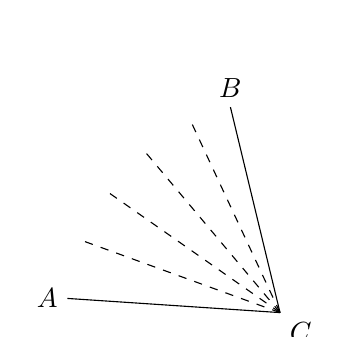
\begin{tikzpicture}[scale=0.9]
  \coordinate (C) at (0,0);
  \coordinate (A) at (-3,0.2);
  \coordinate (B) at (-0.7,2.9);
  \draw (C)--(A);
  \draw (C)--(B);
  \foreach \ang in {115,130,145,160} {\draw[dashed] (C)-- ++(\ang:3);}
  \node[left] at (A) {$A$};
  \node[above] at (B) {$B$};
  \node[below right] at (C) {$C$};
\end{tikzpicture}
\end{center}
% ---- printed p.23 (PDF 28) ----
infinite is thus, both as the infinitely great and the infinitely small, enclosed
by finite limits. But if the infinite is really enclosed by finite limits, then it
must surely, says sound understanding, in one way or another be itself finite.

How does this now really hang together? As guiding examples we may for once
consider the trigonometric functions.
\[
AB = f_1(x) = \sin x;\quad BC = f_2(x) = \cos x;\quad
DF = f_3(x) = \operatorname{tg} x,\quad EG = f_4(x) = \cot x \ \text{etc.}
\]

% FIGURE (printed p.23): unit circle, centre C; horizontal radius CD, vertical
%   radius CE; radius CA at angle x extended through F (on the vertical tangent
%   at D) to G (on the horizontal tangent at E); B = foot of perpendicular from A.
%   AB = sin, CB = cos, DF = tg, EG = cot.
\begin{center}
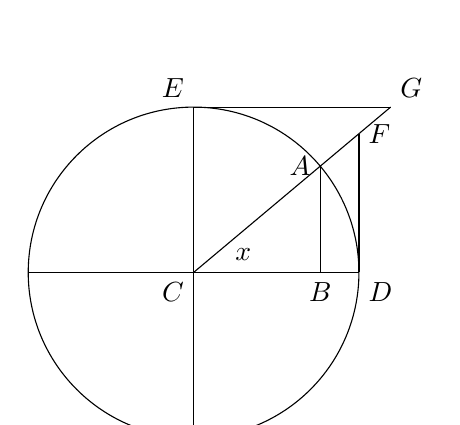
\begin{tikzpicture}[scale=2.1]
  \coordinate (C) at (0,0);
  \coordinate (D) at (1,0);
  \coordinate (E) at (0,1);
  \coordinate (A) at ({cos(40)},{sin(40)});
  \coordinate (B) at ({cos(40)},0);
  \coordinate (F) at (1,{tan(40)});
  \coordinate (G) at ({1/tan(40)},1);
  \draw (C) circle (1);
  \draw (-1,0)--(1,0);
  \draw (0,-1)--(0,1);
  \draw (C)--(G);
  \draw (A)--(B);
  \draw (D)--(F);
  \draw (E)--(G);
  \node at ({0.32*cos(20)},{0.32*sin(20)}) {$x$};
  \node[below left] at (C) {$C$};
  \node[below] at (B) {$B$};
  \node[below right] at (D) {$D$};
  \node[above left] at (E) {$E$};
  \node[left] at (A) {$A$};
  \node[right] at (F) {$F$};
  \node[above right] at (G) {$G$};
\end{tikzpicture}
\end{center}

As $x$, our independent variable, grows in the first quadrant, there grow with it,
as is well known, $\sin$, $\operatorname{tg}$, $\sec$, whereas $\cos$,
$\operatorname{cotg}$, $\operatorname{cosec}\ldots$ decrease. The changes in $x$
proceed, in the first quadrant, from $0^{\circ}$ to $90^{\circ}$; it is necessary
to consider these changes more closely.

If $x = 0$, then $\sin x = 0$, but $\cos x = 1$; $\operatorname{tg} x = 0$, but
$\cot x = \infty$, $\sec x = 1$, but $\operatorname{cosec} x = \infty$; if
$x = 90^{\circ}$, then $\cos x = 0$, $\sin x = 1$, $\operatorname{tg} = \infty$,
$\cot x = 0$, etc.

The finite and the infinite are here determined by one another in such a way that
the transition from finite to finite coincides with the transition from finite to
infinite, whereby then also a transition from finite to $0$ coincides with a
transition from finite to $\infty$.

What does the expression $\angle x = 0$ mean? In the finite sense it might mean
that here there was no $x$ at all; but in virtue of the concept of function
$\angle x = 0$ means a Not-Being which is nevertheless a Being. That an angle
$= 0$ is no angle goes without saying; that $\angle x = 0$ is nevertheless regarded
as being is seen from the fact that a cosine can only be the cosine of an angle,
and that $\cos 0$ is just as surely a real magnitude as $\cos 1^{\circ}$.
% ---- printed p.24 (PDF 29) ----
% FIGURE (printed p.24): a detail of the circle — centre C, horizontal radius to
%   D, two close rays CA and CD' rising to the right, angle x = angle DCA.
\begin{center}
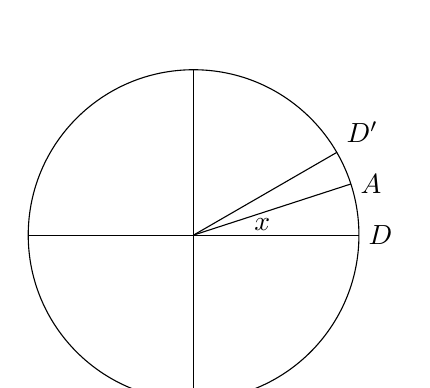
\begin{tikzpicture}[scale=2.1]
  \coordinate (C) at (0,0);
  \draw (C) circle (1);
  \draw (-1,0)--(1,0);
  \draw (0,-1)--(0,1);
  \coordinate (D) at (1,0);
  \coordinate (A) at ({cos(18)},{sin(18)});
  \coordinate (Dp) at ({cos(30)},{sin(30)});
  \draw (C)--(A);
  \draw (C)--(Dp);
  \node at ({0.42*cos(9)},{0.42*sin(9)}) {$x$};
  \node[right] at (D) {$D$};
  \node[right] at (A) {$A$};
  \node[above right] at (Dp) {$D'$};
\end{tikzpicture}
\end{center}

If $A$ is assumed to be at a distance of one degree from $D$ and $D'$, then it
follows that the way from $1^{\circ}$ to $0^{\circ}$ is not longer than the way
from $1^{\circ}$ to $2^{\circ}$. $A$ can come as near to $D$ as one wills; so long
as $A$ does not coincide with $D$, $\angle x$ is a finite magnitude; but the moment
$A$ coincides with $D$, $\angle x$ becomes $= 0$. So long as $x$ is still finite,
$\cot x$ is also finite; but the moment $x$ becomes $= 0$, $\cot x$ becomes
$= \infty$.

The distance from finite to $0$ and from finite to $\infty$ is thus here like a
distance from the one point of finitude to the other. If the one point of finitude
lies infinitely near to the other, then the same can now be said of $0$ and finite,
of $\infty$ and finite.

If, in order to illuminate the relation between the series and the trigonometric
lines, one would fetch an analogy from aesthetics, one would have to say: the
trigonometric functions are classical, the infinite series romantic.

To have the infinite enclosed by the finite is classical; to conceive the infinite
as something beyond the finite, unattainable, romantic. Which of these ways of
viewing does mathematics now support?

In so far as mathematics is an exact science, one would suppose that it held to the
classical; but if we look at its use of categories such as ``approach, infinite
approach'', one would almost believe that it was enthusiastic for the romantic.

With this hint it is naturally not the intention to want to mix the aesthetic into
the mathematical, or to clear up scientific concepts by unscientific analogies. The
fleeting allusion to the aesthetic should merely serve to bring out the difference
between the twofold
% ---- printed p.25 (PDF 30) ----
manner in which the relation of the finite to the infinite is conceived.

What, then, lies in the concept: approach, infinite approach?

By ``infinite approach'' one cannot, in the first place, think of an approach toward
an Attainable; for the Attainable expresses precisely that the approach must end
with the attainment of the goal, and thus be in its essence finite. An approach
toward an Attainable contains no contradiction; an Unattainable without approach is
likewise
% ERRATA APPLIED (from the p.4 „Rettelse."): the print here (p.25, line 9) reads
%   „Tilnærmelse til et Uopnaaeligt indeholder ingen Modsigelse"; the errata
%   directs „læs: Tilnærmelse til et Opnaaeligt". Corrected above to „Opnaaeligt".
no contradiction. There is thus nothing contradictory in the proposition that
parallel lines, however far they be extended, will never intersect one another.
When mathematics sometimes uses the expression, of parallel lines, that they,
extended to infinity, will intersect one another: then one cannot really thereby
think of any approach; it is an impossibility here presented under the form of
possibility.

An infinite approach, an approach toward an Unattainable, on the other hand, seems
to present the hardest of all contradictions. By an approach one must, after all,
in one sense or another come nearer to the goal; but to come nearer to the goal
must surely be the same as to come nearer to the attainment; but from the
attainment of the unattainable one is always equally far away.

None the less, mathematics maintains the concept of an infinite approach, and beats
down every contradiction by incontestable proofs. So in the doctrine of asymptotes.

% FIGURE (printed p.25): a hyperbola branch (solid) and its asymptote (dashed)
%   from A along the axis; ordinates at B and B' meet the curve at D, D' and the
%   asymptote at E, E'. AB = x; BD = y (to the curve); BE = y_1 (to the asymptote).
\begin{center}
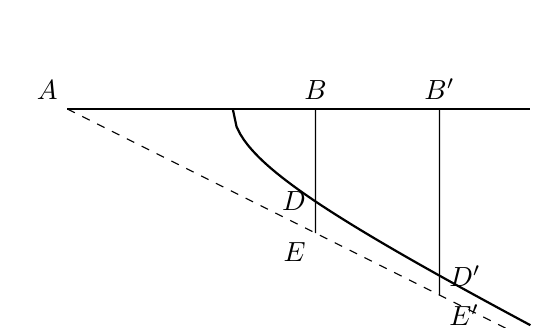
\begin{tikzpicture}[scale=1.05]
  \coordinate (A) at (0,0);
  \draw (A)--(5.6,0);
  \draw[dashed] (0,0)--(5.6,-2.8);
  \draw[thick] plot[domain=2:5.6,samples=80] (\x,{-0.5*sqrt(\x*\x-4)});
  \def\bx{3}\def\bpx{4.5}
  \coordinate (B) at (\bx,0);
  \coordinate (Bp) at (\bpx,0);
  \draw (B)--(\bx,{-0.5*\bx});
  \draw (Bp)--(\bpx,{-0.5*\bpx});
  \coordinate (D) at (\bx,{-0.5*sqrt(\bx*\bx-4)});
  \coordinate (E) at (\bx,{-0.5*\bx});
  \coordinate (Dp) at (\bpx,{-0.5*sqrt(\bpx*\bpx-4)});
  \coordinate (Ep) at (\bpx,{-0.5*\bpx});
  \node[above left] at (A) {$A$};
  \node[above] at (B) {$B$};
  \node[above] at (Bp) {$B'$};
  \node[left] at (D) {$D$};
  \node[below left] at (E) {$E$};
  \node[right] at (Dp) {$D'$};
  \node[below right] at (Ep) {$E'$};
\end{tikzpicture}

$AB = x;\quad BD = y;\quad BE = y_1.$
\end{center}

For the hyperbola one has, for example, the equation:
\[
f(x) = y = \frac{b}{a}\sqrt{x^{2} - a^{2}};
\]
for the hyperbola's asymptote:
% ---- printed p.26 (PDF 31) ----
$f_1(x) = y_1 = \dfrac{b}{a}x$. Accordingly,
\[
\begin{aligned}
y_1 - y &= \frac{b}{a}\left(x - \sqrt{x^{2}-a^{2}}\right)
= \frac{b}{a}\cdot
   \frac{\left(x-\sqrt{x^{2}-a^{2}}\right)\left(x+\sqrt{x^{2}-a^{2}}\right)}
        {x+\sqrt{x^{2}-a^{2}}}\\
&= \frac{b}{a}\cdot\frac{a^{2}}{x+\sqrt{x^{2}-a^{2}}}.
\end{aligned}
\]
The consideration of this formula shows, 1) that here there is a real approach, for
the greater $x$ becomes, the smaller naturally becomes the fraction
$\dfrac{a^{2}}{x+\sqrt{x^{2}-a^{2}}}$; 2) that the goal of the approach is
absolutely unattainable, for the fraction is $0$ only when $x$ has become
$= \infty$.

What validity, then, may we ascribe to the concept of approach?

\begin{center}
  {\bfseries 2)\quad Series with Increasing Powers.}
\end{center}
\phantomsection
\addcontentsline{toc}{subsection}{2) Series with Increasing Powers}

If the concepts ``Unattainable'' and ``approach'' are to be brought into logical
connection, then one might, according to ``\textit{diversus respectus}'', perhaps
begin by thinking of the matter thus: the category ``approach'' must always be
viewed from two standpoints: 1) the point from which one sets out, the point of
departure, and 2) the point that is to be reached, the goal, the end-point.

If there is any movement at all from a definite point of departure toward a goal,
then one may, if the goal is infinitely far away, indeed in one sense grant that
every approach is as a nothing against the infinite remoteness of the goal, and
yet, when one looks back, regard the continued removal from the point of departure
as an approach to the goal. Here, then, in one respect --- namely in so far as one
looks forward --- there is no approach, but yet in another respect --- when, be it
noted, one looks back --- a real approach.

Dialectics could now, to be sure, in this connection very easily confound the
``\textit{diversus respectus}'', and elicit from
% ---- printed p.27 (PDF 32) ----
formal logic the confession that it, according to its own explanation, thus after
all sees the approach only as --- removal, sees forward only in so far as it sees
backward, and that just this is a contradiction; but we have placed ourselves
before the forum of mathematics, and dare not anticipate its verdict.

The inexhaustible possibility of the changes, which lies hidden in the concept of
function as in its ground, steps by the intellectual action out of this ground, and
becomes then, under given conditions, developed in the infinite series.

If a function of $x$ is to be developed, within the limits of finitude, in a series
according to powers, it is natural to begin with the highest power;
\[
\begin{aligned}
f(x) &= x^{n} + A_1 x^{n-1} + A_2 x^{n-2} + A_3 x^{n-3} + \dots A_{n-1}x + A_n\\
&= (x-a_1)(x-a_2)(x-a_3)\dots(x-a_n) = 0,
\end{aligned}
\]
a series with descending powers is then a paradigm.

But when the task is to show how the finite, in infinite approach, strives toward
the infinite, the paradigm must be changed, and the function developed according to
increasing powers:
\[
f(x) = A_0 + A_1 x + A_2 x^{2} + A_3 x^{3} + \dots A_n x^{m} \dots
\]

How such a series can present the infinite approach both to $\infty$ and, in its
separate terms, to $0$, is already clear from the geometric progression.

In the series $a\,\dfrac{1}{1-x} = a + ax + ax^{2} + \dots ax^{n-1}\dots$,
$x^{\infty} = \infty$ if $x > 1$. The series will then not only be capable of being
continued through an infinite number of terms, but with each succeeding term come
ever nearer to $\infty$. For $x < 1$, $x^{\infty} = 0$. The series will thus, by
being continued through countless terms, not only give a greater and greater sum,
but each succeeding term become smaller and smaller, and thus approach $0$.

Mathematics cannot, like formal logic, set itself at rest with an explanation of
``infinite approach'' in
% ---- printed p.28 (PDF 33) ----
words; it uses its sign-language, and articulates the concept, in that for every
infinite series it finds out the relation between the separate terms.

In order that this may happen, the concept of function must assume a definite
character: $f(x)$, for example, $= a^{x}$. One then has the series
$a^{x} = A_0 + A_1 x + A_2 x^{2} + A_3 x^{3} + \dots A_m x^{m} \dots$

For the possible case $a^{x} = a^{0}$, it is easy to determine the series
$a^{0} = A_0$; the rest drops away. But $a^{0} = A_0 = 1$. Since now $f(x) = a^{x}$
is to hold, according to the concept of function, for all possible values of $x$,
one has in this function the first coefficient $A_0 = 1$ determined once for all.

Cartesius's method\footnote{C.\ Ramus. Algbr.\ F.\ S.\ 82. --- The method of
undetermined coefficients. If $f(x) = A_0 + A_1 x + A_2 x^{2} + \dots
= B_0 + B_1 x + B_2 x^{2} + \dots$, then $A_0$ must be $= B_0$, $A_1 = B_1$,
$A_2 = B_2$, and so forth. Proof. For $x = 0$, $A_0 = B_0$ alone remains; by
subtracting $A_0 = B_0$, one obtains $A_1 x + A_2 x^{2} = B_1 x + B_2 x^{2}\dots$,
by dividing by $x$, $A_1 + A_2 x\dots = B_1 + B_2 x$, and, by setting $x = 0$,
$A_1 = B_1$, and so on.} and Newton's binomial formula\footnote{The binomial
formula. From elementary algebra one knows: $(a+b)^{2} = a^{2} + 2ab + b^{2}$;
$(a+b)^{3} = a^{3} + 3a^{2}b + 3ab^{2} + b^{3}\dots$ and so forth. Ram.\ Elmt.\
Algbr.\ S.\ 35. In the higher mathematics (Ramus Algebr.\ Functl.\ S.\ 85) one
presents $(p+x)^{n} = p^{n} + \frac{n}{1}p^{n-1}x + \frac{n(n-1)}{1\cdot 2}
p^{n-2}x^{2} + \frac{n(n-1)(n-2)}{1\cdot 2\cdot 3}p^{n-3}x^{3}\dots$, a series
according to descending powers of $p$ and increasing powers of $x$, whose
coefficients are formed, as the analogy shows, in a manner corresponding to the
exponents of the powers.} give the mathematician, besides, means, as regards the
remaining terms, to bring the variable to merge into the invariable, and, so to
speak, to catch the infinite possibilities in the net of the relations.

% ---- printed p.29 (PDF 34) ----
Thus, in the first place, each coefficient becomes recognizable by the
corresponding power. If, to keep to the given example, the power-factors
$x^{m}z^{n}$ have in the one series the coefficients $A_m A_n$, in the other
$A_{m+n}\dfrac{(m+n)}{1}\dfrac{(m+n-1)\dots(m+1)}{2\cdot 3\dots n}$\footnote{For
one develops, namely, 1) two series according to the same law: $a^{x} = 1 + A_1 x +
A_2 x^{2} + \dots A_m x^{m}\dots$ and $a^{z} = 1 + A_1 z + A_2 z^{2} + \dots
+ A_n z^{n}$, and obtains 2), by multiplying these two equations, two different but
concordant developments: $a^{x}a^{z} = 1 + \dots A_m A_n x^{m}z^{n}\dots$ and
$a^{x+z} = 1 + A_1(x+z) + A_2(x+z)^{2} + \dots A_{m+n}(x+z)^{m+n}\dots$ From the
cited term $A_{m+n}(x+z)^{m+n}$ there is developed again 3) the infinite series:
$A_{m+n}\big[x^{m+n} + \frac{m+n}{1}x^{m+n-1}z +
\frac{(m+n)(m+n-1)}{1\cdot 2}x^{m+n-2}z^{2} + \dots\dots
\frac{(m+n)(m+n-1)(m+n-2)\dots(m+1)}{1\cdot 2\cdot 3\dots n}x^{m}z^{n}\dots\big]$
4) The particular term $A_{m+n}\frac{(m+n)(m+n-1)\dots(m+1)}{1\cdot 2\dots n} =
A_m A_n$.}, then the mathematician has his equation:
\[
A_{m+n}\frac{(m+n)(m+n-1)\dots(m+1)}{1\cdot 2\dots n} = A_m A_n
\]\footnote{The importance of the method of undetermined coefficients one will at
once, among other things, appreciate from this, that the same magnitude can,
without altering its value, present itself not merely under many, but under
infinitely many forms. Among pure magnitudes too there take place --- not, indeed,
intellectual intrigues and mystifications, but yet so many changes of dress,
disguises, and maskings, that he who does not see through the transformations is
easily deceived. How easily, for example, may a beginner be dazzled by the many
terms in the formula $\dfrac{n(n-1)(n-2)\dots(n-n+2)(n-n+1)(n-n)}{1\cdot 2\cdot
3\dots\, n(n+2)\,(n-n+1)}$, so that he does not at once see the masked zero.} and is
assured that it does not deceive. If, then, the mathematician has now on the whole
secured for himself the relation between the powers and their coefficients, then he
uses
% ---- printed p.30 (PDF 35) ----
this relation again to find out thereby the relation between the coefficients among
themselves.

In the cited series, thus, the whole swarm of possible coefficients is brought into
a definite relation to a single one, namely $A_1$, by the formula
$A_m = \dfrac{A_1^{m}}{1\cdot 2\cdot 3\dots m}$\footnote{If one sets:
$A_m A_n = A_{m+n}\dfrac{(m+n)(m+n-1)\dots(m+1)}{1\cdot 2\cdot 3\dots n}$, and
$n = 1$, one gets: $A_m A_1 = A_{m+1}\dfrac{m+1}{1}$, i.e.\
$A_{m+1} = \dfrac{A_m A_1}{m+1}$. If one next sets $m = 1$, one obtains
% print: subscript below reads $A_nA_1$ (should be $A_1A_1$) --- preserved as set
$A_{1+1} = \dfrac{A_n A_1}{1+1} = A_2 = \dfrac{A_1^{2}}{1\cdot 2}$;
if one sets $m = 2$, then one obtains $A_{2+1} = \dfrac{A_2 A_1}{2+1} = A_3 =
\dfrac{A_2 A_1}{3} = \dfrac{\frac{A_1^{2}}{1\cdot 2}A_1}{3} =
\dfrac{A_1^{3}}{1\cdot 2\cdot 3}\dots A_m = \dfrac{A_1^{m}}{1\cdot 2\cdot 3\dots
m}$; from this:
% print oddity: „$a^x = 1 =$" set exactly as here in the original
$a^{x} = 1 = A_1 x + A_2 x^{2} + A_3 x^{3}\dots = 1 +
\frac{A_1 x}{1} + \frac{A_1^{2}x^{2}}{1\cdot 2} +
\frac{A_1^{3}x^{3}}{1\cdot 2\cdot 3} + \dots$
and from this again, when one sets $x = \dfrac{1}{A_1}$;
$a^{\frac{1}{A_1}} = 1 + \frac{A_1}{1}\left(\frac{1}{A_1}\right) +
\frac{A_1^{2}}{1\cdot 2}\left(\frac{1}{A_1}\right)^{2} +
\frac{A_1^{3}}{1\cdot 2\cdot 3}\left(\frac{1}{A_1}\right)^{3} + \dots = 1 +
\frac{1}{1} + \frac{1}{1\cdot 2} + \frac{1}{1\cdot 2\cdot 3} = e$.}; the last,
sole unknown, $A_1$, further brought into a definite relation to $a$ by the
formula: $a^{\frac{1}{A_1}} = 1 + \dfrac{1}{1} + \dfrac{1}{1\cdot 2} +
\dfrac{1}{1\cdot 2\cdot 3}\dots$; this demonstrably converging sum being reckoned
out, and the number found, $e = 2{,}718281828459\dots$, adopted as the base in the
natural, Neperian, logarithmic system.

By the relation between the exponential and the logarithmic function the
coefficient $A_1$ is at last determined in
% ---- printed p.31 (PDF 36) ----
the formula $A_1 = \dfrac{\log a}{\log e}$\footnote{If $a^{\frac{1}{A_1}} = e$, then
$\dfrac{1}{A_1}\log a = \log e$, and $\log a = \log e\, A_1$; thus:
$A_1 = \dfrac{\log a}{\log e}$ ($\log$ here denoting the logarithm in an arbitrary
system).}, a relation which naturally leads again into new relations.

Instead of a logical consideration of the infinite approach in the infinite series,
mathematics thus develops totalities of universally valid and yet peculiar,
infinite and yet definite relations.

How, then, is the relation between the relations and the infinite determined?

\begin{center}
\textbf{3) The Systematics of the Functions.}
\end{center}
\phantomsection
\addcontentsline{toc}{subsection}{3) The Systematics of the Functions}
\markboth{The Problem of Infinity}{The Problem of Infinity}

The problem of infinity is a comprehensive problem of totality; if such a problem
is to be solvable, it must, in the course of continued development, itself bring
with it the conditions of the solution; these conditions must be more closely
investigated.

That the infinite, to recall once more the dialectical, has its limit in the finite
means, then, that it has its determinacy in the finite; that the finite at the same
time has its limit in the infinite must accordingly mean that the determinations of
finitude, by their countlessness, transgress every finite limit.

In the number-relation the finite is now, to be sure, most immediately determined
by the finite; but with the infinite number-relations infinity itself at last
merges into the finite. The unity of the relations and the infinite is at this
stage to be conceived in the concept ``inner infinity''; but the concept ``inner
infinity'' coincides again with the concept of function; the content of infinity
can therefore first unfold itself in the systematic cooperation of the diverse
functions.

% ---- printed p.32 (PDF 37) ----
For the elucidation of the systematics of the functions there must be emphasized
a) that their development can be traced back to one fundamental formula, b) that
their reciprocal relation and mutual transitions point to a common origin, c) that
the one function can, in a continuous series, be developed out of the other.

\begin{center}
\textbf{a) The Fundamental Formula of the Functions.}
\end{center}
\phantomsection
\addcontentsline{toc}{subsubsection}{a) The Fundamental Formula of the Functions}

If one were to attempt to enumerate the possible modes of calculation, rules, and
formulas that occur in mathematical practice, one would soon receive an impression
of a confusing, overwhelming multiplicity, of a boundless finitude that does not
master the infinite. The more, on the contrary, the outwardly manifold is traced
back to the first, general presuppositions, the more the concept prevails, and the
more surveyable the whole becomes.

As a proof of the systematic procedure of mathematics there serves, then, this:
that it not only reduces the countless derived functions to the simplicity of the
fundamental functions, but even refers the development of all functions, elementary
as well as derived, to one fundamental formula. On the condition that one sets, when
required, for example $x+h$ instead of $x$, then
\[
f(x) = A_0 + A_1 x + A_2 x^{2} + A_3 x^{3} + \dots\dots
\]
is a comprehensive fundamental formula.

Under the comprehensive fundamental formula the individuality of the several
functions is as it were veiled; but it is only the finite that is here dissolved, in
order to be grounded in the infinite. With the development the peculiar comes forth
again, and the heterogeneous shows itself. On different conditions the common
possibility becomes, namely, something different, and each function as it steps
forth now sets its own conditions.

For $f(x) = a+x = A_0 + A_1 x + A_2 x^{2} + \dots$, $A_0$ must become $= a$,
$A_1 = 1$, $A_2$, $A_3 \dots = 0$.

For $f(x) = ax = A_0 + A_1 x + A_2 x^{2} + \dots$, $A_0$ must become $= 0$,
$A_1 = a$, $A_2$, $A_3 \dots = 0$.

% ---- printed p.33 (PDF 38) ----
For $f(x) = x^{a} = A_0 + A_1 x + A_2 x^{2}\dots$, likewise only a single term
acquires significance if $x$ is monomial; if $x$ is binomial, for example $= y+z$,
the series reproduces the binomial formula.

For $f(x) = a^{x} = A_0 + A_1 x + A_2 x^{2}\dots$ the definite expression is already
given (S.\ 28).

For $f(x) = \log x = A_0 + A_1 x + A_2 x^{2}\dots$\footnote{If the fractional
exponents are taken into consideration, various alterations again enter in $a^{x}$
and $\log x$.} a series-expansion cannot take place if $x$ is monomial. Since
$\log 0 = \pm\infty$, then, if $x$ were 0, the first term $A_0$ would already be
$= \infty$, and annihilate the significance of the series. If, on the other hand,
one sets $1+x$ instead of $x$, one obtains:
\[
\log(1+x) = \log e\left(x - \frac{x^{2}}{2} + \frac{x^{3}}{3} - \frac{x^{4}}{4}
+ \dots\right)
\]\footnote{Jvfr.\ Ramus.\ Algebr.\ og Funct.\ S.\ 87--88; further elucidation
under b.}

If the trigonometric functions $\cos x$ and $\sin x$ are here added, and it is
recalled that $\cos(-x) = \cos x$, and $\sin(-x) = -\sin x$, ($\cos 0 = 1$ and
$\sin 0 = 0$), then the peculiarity will at once show itself, that $\cos x$ can
contain only even, and $\sin x$ only odd powers of $x$. One then obtains:\footnote{Anf.\
Skr.\ S.\ 88--90.
1) $\cos x = 1 + A_1 x + A_2 x^{2} + A_3 x^{3} + A_4 x^{4}\dots$ ($\cos 0 = 1$,
thus: $A_0 = 1$)
$\cos(-x) = 1 - A_1 x + A_2 x^{2} - A_3 x^{3} + A_4 x^{4}\dots$ ($-x$ gives, in
odd powers, minus, in even, plus).
But $\cos(-x) = \cos x$; if the 2 series are to be equal, $+A_1 = -A_1$,
$+A_3 = -A_3\dots$, then the coefficients with odd indices must all be 0.
If, in the presentation of the series for $\sin x$, one uses $B$ instead of $A$,
thus $\sin x = B_0 + B_1 x + B_2 x^{2} + B_3 x^{3}\dots$, one obtains, since
$\sin 0 = 0$, and $B_0$ consequently $= 0$, $\sin x = B_1 x + B_2 x^{2} +
B_3 x^{3}\dots$, $(\alpha)$, and $\sin(-x) = -B_1 x + B_2 x^{2} - B_3 x^{3} +
B_4 x^{4}\dots$ $(\beta)$; but $\sin(-x) = -\sin x$ (Ramus.\ Trigonometri S.\
8.), and according to $(\alpha) = -B_1 x - B_2 x^{2} - B_3 x^{3}\dots$ In order that
the series $(\alpha)$ for $-\sin x$ may agree with $(\beta)$ for $\sin(-x)$, $B_2$,
$B_4\dots$ must be 0.
2) From the cited series one procures oneself $\alpha)$ a development for
$\cos x\cdot\cos z$, in which there occurs a term $A_m A_n x^{m}z^{n}$,
$\beta)$ a development for $\sin x\sin z$, in which there occurs a term
$B_p B_q x^{p}z^{q}$, and $\gamma)$ from trigonometry (Ramus.\ Trig.\ S.\ 9.) the
two equations: $\cos x\cdot\cos z = \frac{1}{2}\big(\cos(x+z) + \cos(x-z)\big)$ and
$\sin x\cdot\sin z = \frac{1}{2}\big(\cos(x-z) - \cos(x+z)\big)$, and then obtains
from the series for cosine: $A_m A_n = A_{m+n}\frac{(m+n)(m+n-1)\dots(m+1)}{1\cdot
2\cdot\dots\cdot n}$, and from the series for sin, compared with the equations for
cos, $B_p B_q = -A_{p+q}\frac{(p+q)(p+q-1)\dots(p+1)}{1\cdot 2\dots q}$.
3) The relations given lead to definite expressions for the coefficients, namely in
the series for cosine: $A_m = \frac{(-1)^{\frac{m}{2}}}{1\cdot 2\dots m}$,
$A_2 = -\frac{1}{2}$; in the series for sine: $B_p =
\frac{(-1)^{\frac{p+3}{2}}}{1\cdot 2\dots p}$, $B_1 = +1$. In the cosine series one
then has $A_2 = -\frac{1}{2}$, $A_4 = \frac{(-1)^{\frac{4}{2}}}{1\cdot 2\cdot 3\cdot 4}
= \frac{+1}{1\cdot 2\cdot 3\cdot 4}$, $A_6 = \frac{(-1)^{\frac{6}{2}}}{1\cdot
2\cdot 3\cdot 4\cdot 5\cdot 6} = \frac{-1}{1\cdot 2\cdot 3\cdot 4\cdot 5\cdot 6}$;
in the sine series: $B_1 = 1$, $B_3 = \frac{(-1)^{\frac{3+3}{2}}}{1\cdot 2\cdot 3} =
\frac{-1}{1\cdot 2\cdot 3}$, $B_5 = \frac{(-1)^{\frac{5+3}{2}}}{1\cdot 2\cdot
3\cdot 4\cdot 5} = \frac{+1}{1\cdot 2\cdot 3\cdot 4\cdot 5}\dots$}
\[
\cos x = 1 + A_2 x^{2} + A_4 x^{4} + A_6 x^{6}\dots
\]
\[
\sin x = A_1 x + A_3 x^{3} + A_5 x^{5}\dots
\]

% ---- printed p.34 (PDF 39) ----
The peculiarity with which these functions step forth from the fundamental formula
naturally also makes itself known in the result of the development:
\[
\cos x = 1 - \frac{x^{2}}{1\cdot 2} + \frac{x^{4}}{1\cdot 2\cdot 3\cdot 4}
- \frac{x^{6}}{1\cdot 2\cdot 3\cdot 4\cdot 5\cdot 6}\dots
\]
\[
\sin x = x - \frac{x^{3}}{1\cdot 2\cdot 3} + \frac{x^{5}}{1\cdot 2\cdot 3\cdot
4\cdot 5} - \frac{x^{7}}{1\cdot 2\cdot 3\cdot 4\cdot 5\cdot 6\cdot 7}\dots
\]
When one fundamental law thus divides itself into different laws of development, of
which each can again be regarded as a separate fundamental law for new laws of
development, each of these again
% ---- printed p.35 (PDF 40) ----
for new ones, and so forth, there is seen in the connection the systematic, and in
the systematic connection the manner in which the finite relations become
determinations for the infinite. Here shows itself the difference between system and
schema. A schema gives only finite rubrics, but a systematic development proceeds
from the inner infinity of the matter.

\begin{center}
\textbf{b) The Reciprocal Relation of the Functions.}
\end{center}
\phantomsection
\addcontentsline{toc}{subsubsection}{b) The Reciprocal Relation of the Functions}

In a schema nominal definitions hold, but motivated conceptual transitions in a
system.

As an exact science, mathematics gives not merely exact definitions, but shows
besides how the concepts form themselves, and how they operate. It is not the
definition of a logarithm that teaches us what a logarithm is; we learn it
provisionally, in that we see the connection in which the concept arises; we learn
it thoroughly when we see the logarithmic function in its manifold transitions, in
the consequences of its all-sided development.

In a schema mechanical division prevails, but in a system organic articulation.

As an exact science, mathematics maintains exact divisions; one may think of the
division of the elementary functions into simple and composite, algebraic and
transcendent, and the like. But the functions thus divided are not held fast within
the finite limits of measured-out rubrics. One sees from the operations that the
limit is transgressed, and yet precisely maintained, in that it is transgressed.

This holds, for example, of the limit between transcendent and algebraic equations.
$a^{x} = b^{y}$ is transcendent; but through $x\log a = y\log b$ there takes place a
transition to $y = \dfrac{x\log a}{\log b}$, which is algebraic.

The same holds of the limit between the exponential function and the logarithmic. In
the series for the
% ---- printed p.36 (PDF 41) ----
exponential function the coefficient $A_1$ was (II,\ 2) determined by a logarithmic
expression, namely $A_1 = \dfrac{\log a}{\log e}$; one obtains, then:
\[
a^{x} = 1 + \frac{\log a}{\log e}\,x + \left(\frac{\log a}{\log e}\right)^{2}
\frac{x^{2}}{1\cdot 2} + \left(\frac{\log a}{\log e}\right)^{3}\frac{x^{3}}{1\cdot
2\cdot 3} + \dots
\]
Since now the logarithm of the base is always 1, one chooses the system whose base
is $e = 2{,}718281828459\dots$, and, denoting the logarithm in this system by $l$,
there results
\[
a^{x} = 1 + (l.\,a)\,x + (l.\,a)^{2}\frac{x^{2}}{1\cdot 2} + (l.\,a)^{3}
\frac{x^{3}}{1\cdot 2\cdot 3}\dots\dots
\]
One thus not only passes, within the limit of the logarithm-category, over from the
one system into the other; but one applies the logarithm-category in order to make
clear to oneself the power-category: the value of an exponential function is asked
for, and answered with the value of a logarithmic one; the value of the logarithmic
function is asked for, and answered with the value of the exponential.\footnote{The
equation cited under a):
$\log(1+x) = \log e\left(x - \frac{x^{2}}{1\cdot 2} + \frac{x^{3}}{1\cdot 2\cdot
3} - \frac{x^{4}}{1\cdot 2\cdot 3\cdot 4}\dots\right)$
% print: denominators here are $1\cdot2,\,1\cdot2\cdot3,\dots$ --- differ from the p.33 statement ($/2,/3,/4$)
is developed thus: 1) $(1+x)^{y} = 1 + \frac{y}{1}x +
\frac{y(y-1)}{1\cdot 2}x^{2} + \frac{y(y-1)(y-2)}{1\cdot 2\cdot 3}x^{3}\dots$
2) $(1+x)^{y} = 1 + \frac{\log(1+x)}{\log e}y +
\log\left(\frac{1+x}{\log e}\right)^{2}\frac{y^{2}}{1\cdot 2}\dots$
% print: 2nd expansion's 3rd term is set „$\log(\frac{1+x}{\log e})^2$" --- evidently for $(\frac{\log(1+x)}{\log e})^2$
by ordering these series according to increasing powers of $y$, and then comparing
them.}

The same holds of the limit between the exponential function and the trigonometric
ones.

If in the equation $a^{x} = 1 + (l.\,a)x + (l.\,a)^{2}\frac{x^{2}}{1\cdot 2}
+ (l.\,a)^{3}\frac{x^{3}}{1\cdot 2\cdot 3} + \dots$ one sets $e$ instead of $a$, and
recalls that $l.\,e = 1$, one obtains:
\[
e^{x} = 1 + \frac{x}{1} + \frac{x^{2}}{1\cdot 2} + \frac{x^{3}}{1\cdot 2\cdot 3}
+ \dots
\]
% ---- printed p.37 (PDF 42) ----
If in this equation one sets $x\sqrt{-1}$ instead of $x$, one obtains:
\begin{multline*}
e^{x\sqrt{-1}} = 1 + \frac{x\sqrt{-1}}{1} + \frac{(x\sqrt{-1})^{2}}{1\cdot 2}
+ \frac{(x\sqrt{-1})^{3}}{1\cdot 2\cdot 3} + \frac{(x\sqrt{-1})^{4}}{1\cdot 2\cdot
3\cdot 4}\dots \\
= 1 + x\sqrt{-1} - \frac{x^{2}}{1\cdot 2} - \frac{x^{3}\sqrt{-1}}{1\cdot 2\cdot 3}
+ \frac{x^{4}}{1\cdot 2\cdot 3\cdot 4}\dots
\end{multline*}
for the powers of $\sqrt{-1}$ form a period of 4 terms: $\sqrt{-1}$, $-1$,
$-\sqrt{-1}$, and $+1$, which repeat themselves to infinity.

If one now multiplies the equation $\sin x = x - \frac{x^{3}}{1\cdot 2\cdot 3} +
\frac{x^{5}}{1\cdot 2\cdot 3\cdot 4\cdot 5} - \frac{x^{6}}{1\cdot 2\cdot 3\cdot
4\cdot 5\cdot 6} + \dots$
% print: 4th term numerator set $x^{6}$ (should be $x^{7}$; cf. the same series on p.34)
by $\sqrt{-1}$, one obtains $\sin x\sqrt{-1} = x\sqrt{-1} -
\frac{x^{3}\sqrt{-1}}{1\cdot 2\cdot 3}\dots$, which value corresponds precisely to
the 2nd and 4th terms, and so forth, in the series for $e^{x\sqrt{-1}}$, while the
value for $\cos x$, namely $1 - \frac{x^{2}}{1\cdot 2} + \frac{x^{4}}{1\cdot 2\cdot
3\cdot 4}$, corresponds to the 1st, 3rd, and 5th terms, and so forth.

Thus, in $e^{x\sqrt{-1}} = \cos x + \sqrt{-1}\sin x$, and, when one sets
$-x\sqrt{-1}$ instead of $x\sqrt{-1}$, in $e^{-x\sqrt{-1}} = \cos x - \sqrt{-1}\sin x$,
the exponential function is expressed by the trigonometric; from which it further
follows that the trigonometric can likewise be expressed by the logarithmic. For if
$e^{x\sqrt{-1}} = \cos x + \sqrt{-1}\,s\,n\,x$,
% print: „s n x" set thus (typo for sin x)
then also $x\sqrt{-1} = l.\,(\cos x + \sqrt{-1}\sin x)$\footnote{``The
trigonometric lines are, as functions of the circular arc, reducible to the
exponential function, and the circular arc, as a function of the trigonometric
lines, reducible to the logarithm.'' Ramus.\ Algbr.\ Functsl.\ S.\ 15.}.

% ---- printed p.38 (PDF 43) ----
The systematic intercourse between the exponential function and the trigonometric
ones is thus brought about by the application of an imaginary magnitude, $\sqrt{-1}$;
but an imaginary magnitude belongs, according to the definition, to the impossible.
By the in-itself impossible, then, a real reduction has become possible: how is this
now to be understood?

If anyone should answer: $\sqrt{-1}$ is both impossible and yet possible; then formal
logic would perhaps interpret the answer thus: $\sqrt{-1}$ is in one respect
impossible, in so far, namely, as there is here required a number which, raised to
the 2nd power, should give $-1$, in another respect, on the contrary, possible, in
that one, by, for example, raising $\sqrt{-1}$ to the 2nd power, obtains a real
magnitude, $-1$. This might then be an example of the maxim: \textit{diversus
respectus tollit omnem contradictionem}.

But with all respect for \textit{diversus respectus}, such a resolution of the
contradiction is nevertheless only formal, and the merely formal is the superficial.
With this superficiality science cannot set itself at rest: mathematics proceeds to
operations; philosophy follows after, and looks at the dialectical.

If one could, with the logical maxim \textit{possibile est, quod non implicat
contradictionem}, as regards the concepts, keep to nominal definitions, one would
soon be done with the separation of the possible and the impossible\footnote{In this
way a round quadrangle would indeed be impossible, but hardly a regular
heptahedron.}; but a thorough separation is conditioned by systematics.

Mathematics teaches us, when we follow its systematic development, that much is
possible which at first glance seems impossible, and, conversely, much at bottom
impossible which an uninitiated person easily takes for possible.

% ---- printed p.39 (PDF 44) ----
Yes, so dialectical is the limit of possibility, even in the mathematical domain,
that the exact science itself in many points is still scarcely able to hold it
fast.\footnote{In order not to dwell on questions such as: is it possible to find a
comprehensive law for the determination of the prime numbers? is it possible to find
a finite solution for the general equation of the $n$th degree? is it absolutely
impossible to bring the quadrature of the circle under a finite expression,
absolutely impossible that $\pi$ can be periodic? and so forth --- we will in this
connection bring out a little more closely the dispute concerning the imaginary
magnitudes. Thus: 1) is $\sqrt{-1}$ an absolute impossibility? Since $(-a)$ is
produced from $(+a)$ by multiplying this magnitude by $(-1)$, one can make clear to
oneself the meaning of this multiplication by rotations.
% FIGURE (printed p.39, embedded within this footnote *): coordinate cross —
%   real axis A(left)--B(right) with -a, +a; imaginary axis C(bottom)--D(top)
%   with -b, +b; origin at Coordinatsystemets Begyndelsespunkt. Redrawn in TikZ.
\begin{center}
\begin{tikzpicture}[scale=0.5]
  \draw (-2.4,0) -- (2.4,0);
  \draw (0,-2.4) -- (0,2.4);
  \node[left] at (-2.4,0) {$A$};
  \node[right] at (2.4,0) {$B$};
  \node[above] at (0,2.4) {$D$};
  \node[below] at (0,-2.4) {$C$};
  \node[below] at (-1.2,0) {$-a$};
  \node[below] at (1.2,0) {$+a$};
  \node[right] at (0,1.2) {$+b$};
  \node[right] at (0,-1.2) {$-b$};
\end{tikzpicture}
\end{center}
A rotation of $90^{\circ}$ is then denoted by $+a\sqrt{-1}$; of $180^{\circ}$
by $+a\sqrt{-1}\sqrt{-1} = a(-1) = -a$; of $270^{\circ}$ by
$a(-1)\sqrt{-1} = -a\sqrt{-1}$; of $360^{\circ}$ by
$-a\sqrt{-1}\sqrt{-1} = -a(-1) = +a$. But then one must, to be sure, combine such
heterogeneous concepts as multiplication and rotation. If one has, the origin of the
coordinate system being at the centre,
$\frac{x^{2}}{a^{2}} + \frac{y^{2}}{b^{2}} = 1$ as the equation of the ellipse, then
one can, by setting $b = \sqrt{-1}\,b'$, and consequently $b^{2} = -{b'}^{2}$, obtain:
$\frac{x^{2}}{a^{2}} - \frac{y^{2}}{{b'}^{2}} = 1$, which is the equation of the
hyperbola. The impossible and therefore imaginary $\sqrt{-1}$ thus becomes, after
all, in a way real, and therefore possible. 2) Are logarithms of negative magnitudes
possible? On a fleeting consideration it should seem as if there were nothing in the
way. One has $\log(a^{2}) = 2\log a$, and $\log(-a)^{2} = \log(a^{2})$; how near,
then, lies the conclusion that $\log(-a)^{2}$ must also be $= 2\log(-a)$, and yet the
conclusion is false. One has, when $a$ and $b$ are positive,
$\sqrt{a}\cdot\sqrt{b} = \sqrt{a\cdot b}$; but since $\sqrt{-a}$ is impossible, the
above equation does not hold for negative magnitudes. One cannot say
$(\sqrt{-a})^{2} = \sqrt{-a}\,\sqrt{-a} = \sqrt{(-a)^{2}} = \sqrt{a^{2}} = \pm a$,
for it is only $\sqrt{-a}$ which, raised to the 2nd power, gives $-a$. In the dispute
against Bernoulli, Leibnitz saw the truth, but lacked the means to disarm his
opponent; in the dispute against d'Alembert, Euler applied the formulas:
$a^{x} = 1 + (l.\,a)\frac{x}{1} + (l.\,a)^{2}\frac{x^{2}}{1\cdot 2} + \dots$,
$e^{x\sqrt{-1}} = \cos x + \sin x\sqrt{-1}$, and
$l(\cos x + \sin x\sqrt{-1}) = x\sqrt{-1}$, and found in these formulas points of
departure for clear proofs. For if one sets the formula:
$e^{(2p\pi+y)\sqrt{-1}} = \cos(2p\pi+y) + \sin(2p\pi+y)\sqrt{-1}$, $p =$ any
whole number whatever; and sets further $a = r\cos(2p\pi+y)$,
$b = r\sin(2p\pi+y)$, one obtains, by the roundabout way of the reductions (jvfr.\
Ramus.\ Algbr.\ Functsl.\ S.\ 92--94), the following formulas for comparison:
% l^{1}, p^{1}, p^{11} are the raised „1"/„11" set in the print (principal-log
%   branch and integer indices) --- reproduced as printed.
(I) $l.\,a^{2} = l^{1}a^{2} + 2p\pi\sqrt{-1}$;
(II) $l.\,a^{2} = 2l^{1}a + 2p\pi\sqrt{-1}$;
(III) $2l.\,a = 2l^{1}a + 4p^{1}\pi\sqrt{-1}$ (in that the equation
$l.\,a = l^{1}a + 2p^{1}\pi\sqrt{-1}$ is multiplied by 2);
(IV) $2l(-a) = 2l^{1}(a) + 2(2p^{11}+1)\pi\sqrt{-1}$ (since one has
$l(-a) = l^{1}a + (2p^{11}+1)\pi\sqrt{-1}$). If IV is compared with III, then
$2l(-a) = 2l(a)$ when $4p^{1} = 2(2p^{11}+1)$, or when $2p^{1} = 2p^{11}+1$;
but this is impossible, since an even number can never become equal to an odd one.
According to the other comparisons one finds that the terms which $l(-a)$ has in
common with $l.\,a$ in the infinite series are altogether imaginary. A real logarithm
of $-a$ is thus, after all, an impossibility.}

% ---- printed p.40 (PDF 45) ----
That the limits are maintained in that they are transgressed shows, moreover, how
definitions and transitions, mechanical division and infinite articulation, condition
one another in a scientific system. In so far as the several functions are placed as
if in rubrics side by side, and held against one another, they are placed
realistically: the more firmly the finite opposition is held, the
% ---- printed p.41 (PDF 46) ----
stronger is the realism. Mathematical practice, however, itself subdues this realism,
in that it lets each of the separated functions take up the others into its
self-development. Each function thus returns, through the others, into itself, has
thus the others as moments in its determination of concept and its content; this is
the idealistic. For the realist the relations are finite, for the idealist they are
infinite: in a carried-through systematics the finite relations become grounded in
the infinite.

\begin{center}
\textbf{c) Taylor's Series.}
\end{center}
\phantomsection
\addcontentsline{toc}{subsubsection}{c) Taylor's Series}

The systematic connection of finite terms, which articulates the inner infinity, is
in all points immediate and yet infinitely mediated.

If, however, anyone should say: ``our cognition is thus immediate only because it is
so infinitely mediate'', such an utterance would easily be taken as a proof of
subtlety and dialectical wordplay.

Yet the validity of the proposition set up will precisely become immediately evident,
once the understanding has first been mediated.

In a chain of material links it holds, to be sure, that while the first and second
links are in immediate connection, the first and third links are only in a mediate,
the first and fourth in a still more mediate connection. But with such a
parcelling-out of the immediate and the mediate the concept ``inner infinity'' is
incompatible.

In the intellectual connection one speaks, to be sure, also of the connection of the
extreme terms by middle terms; but the deeper the insight goes, the more the finite
middle terms, as determinations of concept, are dissolved in the intimate unity of
the extreme terms.

In order not to be dazzled by the mediacy in the entering middle terms, one must look
at the light-effect, and make clear to oneself the difference between the transparent
and the non-transparent.

% ---- printed p.42 (PDF 47) ----
As regards the sensible light-effect, it is the obscurity of the middle terms, the
finitude of the means, that lets us feel the mediate.

He who would know figures that move behind a partition-wall must by a roundabout way
procure himself information, and thereby marks the mediate. If now it is not a wall,
but a translucent pane, that separates the beholder from the objects, the mediate
already begins to disappear: he sees the shadows move immediately, although the pane
is perceived as a distancing middle term. If the pane is of purely transparent glass,
the middle term does not trouble at all; and if the eye is armed besides with the
glass of the telescope, then we have here an example of middle terms which, instead
of removing the corresponding extreme terms, the beholder and the object, on the
contrary bring them nearer to one another, and, instead of binding them by the
mediate, even let them meet in heightened immediacy.

If the presupposition in question is evident, then its nearest consequence is also
evident. Once one has understood what is meant by
$A_m A_n = A_{m+n}\dfrac{(m+n)(m+n-1)\dots(m+1)}{1\cdot 2\cdot 3\dots n}$, then it is
also immediately evident that $A_m A_1$ must be, for $n = 1$,
$= A_{m+1}\dfrac{m+1}{1}$; if the equation $A_m A_1 = A_{m+1}\dfrac{m+1}{1}$ is
immediately evident, then the equation $A_{m+1} = \dfrac{A_m A_1}{m+1}$ is also
immediately evident.

But thus it stands with all transitions in the higher as in the lower mathematics.
Each proposition must, in its peculiar connection, be immediately evident, and yet in
this peculiar connection there is precisely the mediate. The more the connection is
cleared up, the more transparent the middle terms become, the more, therefore, will
the mediate also merge into higher immediacy.

% ---- printed p.43 (PDF 48) ----
For the mathematically educated it is just as easy to run through the proof of
$A_m A_n = A_{m+n}\dfrac{(m+n)(m+n-1)\dots(m+1)}{1\cdot 2\cdot 3\dots n}$ in the
above-cited connection, as for the beginner to understand the inference: $A > B$,
$B > C$, thus $A > C$.

If we consider the equation:
\[
f(x+h) = A_0 + A_1(x+h) + A_2(x+h)^{2} + A_3(x+h)^{3}\dots
\]
as an infinite chain of finite terms, then it can be proved that in such a chain
there is the possibility of an infinite mediation of the connection of the terms. The
method, the way of mediation, is at once a roundabout way and a short cut.

Since $f(x+h)$ is not yet more closely determined, one can, in the first place, set
the condition that the otherwise undetermined coefficients $A_0$, $A_1$, $A_2\dots$
shall be functions, namely different functions of $x$, not of $h$, and, to recall the
fulfilment of the condition, write the series thus:
\[
f(x+h) = f(x) + f_1(x)h + f_2(x)h^{2} + f_3(x)h^{3} + \dots f_m(x)h^{m} + \dots
= X_0 + X_1 h + X_2 h^{2} + X_3 h^{3}\dots + X_m h^{m}\dots
\]

In order to secure for ourselves an all-sided systematic connection, we set, in the
second place, the condition that the infinite series be developed in such a way that
its terms can again be developed in infinite series.

In order that this condition may be fulfilled, we introduce, in the third place,
besides $h$ still an increment $k$, and thereby procure for ourselves a double
development, in that $k$ is on the one side added to $h$, on the other side to $x$.

Finally, in the fourth place, the condition must still be added, that the function be
so chosen that one expressly obtains:
$f(x + \overline{h+k}) = f(\overline{x+k} + h)$.

These, then, are our nearest presuppositions; we shall now test the consequences of
these presuppositions.

In the series (I):
\[
f(x + \overline{h+k}) = X_0 + X_1(h+k) + X_2(h+k)^{2} + \dots
X_{m+n}(h+k)^{m+n}\dots
\]
there can, from the last-cited term, be developed an
% ---- printed p.44 (PDF 49) ----
infinite series which, among its countless terms, must contain the following:
\[
X_{m+n}\frac{(m+n)(m+n-1)\dots(m+1)}{1\cdot 2\dots n}
\]
In the series (II), with its series:
\[
\begin{aligned}
f(\overline{x+k}+h) = {}& f(x+k)\,(= X_0 + X_{0,1}k + X_{0,2}k^{2}\dots
X_{0,n}k^{n}\dots)\\
+{}& f_1(x+k)h\,(= X_1 h + X_{1,1}hk + \dots X_{1,n}hk^{n}\dots)\\
+{}& f_2(x+k)h^{2}\,(= X_2 h^{2} + X_{2,1}h^{2}k \dots X_{2,n}h^{2}k^{n}\dots)\\
&\ \ \vdots\\
+{}& f_m(x+k)h^{m}\,(= X_m h^{m} + X_{m,1}h^{m}k + \dots X_{m,n}h^{m}k^{n}\dots)
\end{aligned}
\]
one has, then, $X_{m,n}h^{m}k^{n}$, according to the method of undetermined
coefficients,
\[
= X_{m+n}\frac{(m+n)(m+n-1)\dots(m+1)}{1\cdot 2\dots n}.
\]
In such combinations the mediate prevails: the way of the method is a roundabout way.

That now this roundabout way is precisely a short cut, in that the extreme terms,
distanced by middle terms, are brought infinitely near to one another, can in this
connection just as easily be demonstrated:

One has, according to (I), $X_1(h+k) = X_1 h + X_1 k$, and, according to (II),
$X_{0,1}k$, and thus, according to the method of undetermined coefficients,
$X_{0,1} = X_1$; from this it is seen that $X_{m,1}$ arises from $X_m$ in the same way
as $X_{0,1} = X_1$ from $X_0$.

If one now sets $X_0 = f(x)$, and $X_1 = \dfrac{f'(x)}{1}$, then one obtains, for
$m = 1$, $= 2, \dots = n, \dots$
\begin{align*}
X_{1+1} &= X_2 = \frac{X_{1,1}}{2} = \frac{\frac{f''(x)}{1}}{2}
= \frac{f''(x)}{1\cdot 2}\\
X_{2+1} &= X_3 = \frac{X_{2,1}}{3} = \frac{\frac{f'''(x)}{1\cdot 2}}{3}
= \frac{f'''(x)}{1\cdot 2\cdot 3}\\
X_n &= \frac{X_{n-1,1}}{n} = \frac{f^{n}(x)}{1\cdot 2\dots n}
\end{align*}

% ---- printed p.45 (PDF 50) ----
If, then, one knows the manner in which $X_1$ arises from $X_0$, one knows at the
same time the manner in which each succeeding term arises from its preceding one. If
the relation between the first and second terms is evident, then at the same time the
relation between the first and third, first and fourth, first and thousandth terms
becomes evident. The short cut is conditioned by this, that the mediacy is raised to
higher immediacy --- in the depth of insight.

If now the coefficients are, on the conditions given, determined as functions of $x$,
the series:
\[
f(x+h) = f(x) + f_1(x)h + f_2(x)h^{2} + f_3(x)h^{3} + \dots f_m(x)h^{m}\dots
\]
can be written:
\[
f(x+h) = f(x) + f'(x)\frac{h}{1} + f''(x)\frac{h^{2}}{1\cdot 2}
+ f'''(x)\frac{h^{3}}{1\cdot 2\cdot 3} + \dots
f^{m}(x)\frac{h^{m}}{1\cdot 2\cdot 3\dots m}\dots
\]
This so-called Taylorian series can, when one, after having produced $f'(x)$,
$f''(x)\dots$ from $f(x)$, sets $x = 0$, and $h = x$, be transformed again into
Maclaurin's series:
\[
f(x) = f(0) + f'(0)\frac{x}{1} + f''(0)\frac{x^{2}}{1\cdot 2} + \dots
f^{m}(0)\frac{x^{m}}{1\cdot 2\cdot 3\dots m}\dots
\]
If, then, we hold fast to the identity of roundabout way and short cut, then a
retrospect now also shows that the infinite mediation of the method is due at once to
the necessary movement of the matter and the free movement of thought.

We have the formula: $a^{x} = 1 + \frac{A_1 x}{1} + \frac{A_1^{2}x^{2}}{1\cdot 2}
+ \frac{A_1^{3}x^{3}}{1\cdot 2\cdot 3}\dots$; it is expressly our task to find $A_1$;
but the definite expression for $A_1$ by no means follows from the formula in the
same way as from $A > B$, $B > C$ follows $A > C$.

The solution of the task is necessarily conditioned by the given connection, but it
is nevertheless thought that sets itself the task, and finds out the way.

% ---- printed p.46 (PDF 51) ----
To set $x = \dfrac{1}{A_1}$ looks at first glance like an ingenious device, for it is
an expedient that freedom has found; but, more closely considered, the expedient is
prescribed. Freedom's choice is grounded in the necessity of the matter.

We have the formulas: $a^{x} = 1 + (l.\,a)x + (l.\,a)^{2}\frac{x^{2}}{1\cdot 2}
+ (l.\,a)^{3}\frac{x^{3}}{1\cdot 2\cdot 3}\dots$ and
$e^{x} = 1 + \frac{x}{1} + \frac{x^{2}}{1\cdot 2} + \frac{x^{3}}{1\cdot 2\cdot 3}
\dots$ The task is to find a systematic connection between the exponential function
and the trigonometric ones. The necessary middle term lies in the matter; but it
takes a Euler to discover the middle term.

We have in the formula:
\[
f(x+h) = A_0 + A_1(x+h) + A_2(x+h)^{2} + A_3(x+h)^{3}\dots
\]
the possibility of countless series-expansions. The conditions that are set, the
directions that are followed, the whole method, are here just as little an immediate
consequence of necessity as a chance product of arbitrariness.

It is the matter that yields the conditions, but free thought that chooses the
conditions; it is the matter that furnishes the presuppositions, but free thought
that orders the presuppositions; it is the matter that supplies the means, but free
thought that fixes the goal. The goal is, in this connection, an analysis of the
infinite.

\begin{center}\rule{2.5cm}{0.4pt}\end{center}

\begin{center}
  {\large\bfseries III.}\par\vspace{4pt}
  {\Large\bfseries The Analysis of the Infinite.}
\end{center}
\phantomsection
\addcontentsline{toc}{section}{\texorpdfstring{III.\quad The Analysis of the Infinite}{III. The Analysis of the Infinite}}
\markboth{The Analysis of the Infinite}{The Analysis of the Infinite}

In the approach toward an Unattainable the problem of infinity first found its
contemplable expression; the inner infinity of the finite relations
% ---- printed p.47 (PDF 52) ----
then showed us the way to the solution of the problem.

That such a solution concerns not only mathematics, but in the highest degree
philosophy, can already be seen from the contradiction in which the knot is tied. The
contradiction is that the infinite is at an unattainable remoteness (the asymptote),
because it is everywhere so infinitely near to the finite (the trigonometric
functions).

If we follow, as hitherto, the mathematical track, the incessant approach is to be
more closely determined by the function-limit, the \emph{Limit}\footnote{Ramus.\
Algbr.\ Funct.\ S.\ 78--79.}, the limit toward which a function of $x$ converges, as
$x$ either increases or decreases to infinity. As regards the, so to speak,
omnipresence of the infinite in the finite, we are then referred to the
\emph{Differential}, the infinitude-difference that arises between $f(x)$ and
$f(x+h)$, when $h$ is regarded as an infinitely small increment to $x$; finally to
the \emph{Integral}, the expression which shows how one, through the roundabout ways
of the infinite, finds the short cut back to the finite.

\begin{center}
\textbf{1) The Function-Limit.}
\end{center}
\phantomsection
\addcontentsline{toc}{subsection}{1) The Function-Limit}

In the equation $\mathrm{Lim}\, f(x) = f(\infty) = c$, $c$ is the value, the limit, to
which $f(x)$ more and more approaches, as $x$ becomes greater and greater --- a limit
which, however, is first attained when $x$ becomes $= \infty$, thus by infinite
approach.

Example:
\[
f(x) = \frac{a + a_1 x + a_2 x^{2} + \dots a_n x^{n}}{b + b_1 x + b_2 x^{2}
+ \dots b_n x^{n}}
\]
So long as $x$ is only a finite magnitude, none of the terms can be thrown away;
however, one can, by dividing by $x^{n}$, transform the whole quotient without
altering its value. Thus:
% ---- printed p.48 (PDF 53) ----
\[
f(x) = \frac{\dfrac{a}{x^{n}} + \dfrac{a_1}{x^{n-1}} + \dfrac{a_2}{x^{n-2}}
+ \dots a_n}{\dfrac{b}{x^{n}} + \dfrac{b_1}{x^{n-1}} + \dfrac{b_2}{x^{n-2}}
+ \dots b_n}
\]
The transformation shows that those terms in numerator and denominator which are
divided by $x$ acquire less and less value, the more $x$ grows. If now one sets
$x = \infty$, one obtains:
\[
f(\infty) = \frac{\dfrac{a}{\infty^{n}} + \dfrac{a_1}{\infty^{n-1}}
+ \dfrac{a_2}{\infty^{n-2}} + \dots a_n}{\dfrac{b}{\infty^{n}}
+ \dfrac{b_1}{\infty^{n-1}} + \dfrac{b_2}{\infty^{n-2}} + \dots b_n}
= \frac{0+0+0+\dots a_n}{0+0+0+\dots b_n} = \frac{a_n}{b_n} = c
\]
In the equation:
\[
\lim f(x) = f(0) = c'
\]
$c'$ denotes the value, the limit, to which the function approaches, as $x$ becomes
smaller, but which is only reached in infinite approach, in so far as it is first
reached when $x = 0$.

Example.
From $f(x) = \dfrac{a + a_1 x + a_2 x^{2} + \dots a_n x^{n}}{b + b_1 x + b_2 x^{2}
+ \dots b_n x^{n}}$ it is seen that all the terms multiplied by $x$ must acquire a
smaller value, the smaller $x$ becomes. If $x$ at last becomes $= 0$, one gets:
\[
f(0) = \frac{a + a_1\cdot 0 + a_2\cdot 0^{2} + \dots a_n\cdot 0^{n}}{b
+ b_1\cdot 0 + b_2\cdot 0^{2} + \dots b_n\cdot 0^{n}} = \frac{a}{b} = c'.
\]
But, one might object, one is so far from yet seeing any difference between
$\infty^{n}$ and $\infty^{1}$, between $0^{n}$ and $0^{1}$, that it even seems as if
$0$ and $\infty$, even when they are introduced by the way of approach, nevertheless
continue to obliterate all difference between the finite, definite magnitudes.

In order to grasp the relativity which the approach introduces into the infinite, we
must consider the infinite magnitudes $0$ and $\infty$, partly in relation to the
finite, partly in relation to one another.
% ---- printed p.49 (PDF 54) ----
\[
a > b; \quad \text{but } a\cdot\infty = b\cdot\infty, \quad a\cdot 0 = b\cdot 0.
\]
\[
\mathrm{Lim}(x) = \infty; \quad \mathrm{Lim}\left(\frac{1}{x}\right)
= \mathrm{Lim}\frac{1000}{x} = 0.
\]
\[
\lim(x) = 0; \quad \lim\frac{1}{x} = \lim\frac{1000}{x} = \infty.
\]
Thus every finite magnitude will, in comparison with the infinitely great, be
vanishing; and likewise the infinitely small will be vanishing in comparison with
every finite magnitude. In so far as the finitude-limit has vanished, $0$ and
$\infty$ still maintain their rank with the infinite; but in so far as the vanished
points back to a vanishing, and this vanishing to the approach, $0$ and $\infty$
descend from the absolute height of infinity, and enter into calculation with finite
magnitudes.

We can make the matter clear thus. In the formula $\frac{x}{x} = 1$, $x$ may well
change, become greater and greater, smaller and smaller, without the quotient in
question changing. $\mathrm{Lim}\frac{x}{x} = \frac{\infty}{\infty}$ is thus no
longer an indeterminate expression, but quite determinately $= 1$; equally
determinate is $\lim\frac{x}{x} = \frac{0}{0} = 1$. What holds of the quotient
$\frac{x}{x'}$,
% print: denominator set $x'$ (a prime) --- cf. the $\frac{x}{x}$ just discussed
holds also of $\frac{x^{2}}{x}$, $\frac{x^{3}}{x}$, $\frac{x^{n}}{x}$, and so
forth. Thus: since $\frac{x^{2}}{x} = x$, $\mathrm{Lim}\frac{x^{2}}{x} =
\frac{\infty^{2}}{\infty} = \infty$, and $\lim\frac{x^{2}}{x} = \frac{0^{2}}{0}
= 0$. Since $\frac{x^{n}}{x} = x^{n-1}$, then $\mathrm{Lim}\frac{x^{n}}{x} =
\frac{\infty^{n}}{\infty} = \infty^{n-1}$, and $\lim\frac{x^{n}}{x} =
\frac{0^{n}}{0} = 0^{n-1}$.

In order to see how the contradiction which lies in the concept of infinite
magnitude is resolved in the mathematical presentation, we can for a moment let the
infinite approach halt at a finite limit. Where this
% ---- printed p.50 (PDF 55) ----
limit is set is, as regards the concept, indifferent, since it is set only in order
to be immediately transgressed.

The magnitude $1{,}000{,}000$ represents for a moment $\infty$; the quotient
$\frac{1}{1{,}000{,}000}$ will then necessarily represent $0$.

In accordance with the above formulas we shall thus obtain:
\begin{gather*}
\frac{1{,}000{,}000}{1{,}000{,}000} = \frac{\infty}{\infty} = 1; \quad
\frac{\frac{1}{1{,}000{,}000}}{\frac{1}{1{,}000{,}000}} = \frac{0}{0} = 1.\\
\frac{(1{,}000{,}000)^{2}}{1{,}000{,}000} = \frac{\infty^{2}}{\infty}
= 1{,}000{,}000 = \infty;\\
\frac{\left(\frac{1}{1{,}000{,}000}\right)^{2}}{\frac{1}{1{,}000{,}000}}
= \frac{0^{2}}{0} = \frac{1}{1{,}000{,}000} = 0.\\
\frac{(1{,}000{,}000)^{3}}{1{,}000{,}000} = \frac{\infty^{3}}{\infty}
= 1{,}000{,}000^{2} = \infty^{2};\\
\frac{\left(\frac{1}{1{,}000{,}000}\right)^{3}}{\frac{1}{1{,}000{,}000}}
= \frac{0^{3}}{0} = \left(\frac{1}{1{,}000{,}000}\right)^{2} = 0^{2}
\end{gather*}
The objection that $1{,}000{,}000$ is infinitely far from $\infty$, and
$\frac{1}{1{,}000{,}000}$ consequently equally far from $0$, means nothing; since the
finitude-limit is set only in order to be transgressed, one will not only be able to
let $1{,}000{,}000^{1{,}000{,}000}$ instead of $1{,}000{,}000$ represent $\infty$,
but --- what is here decisive --- also see that the terms of the relation can be
changed to infinity, without the definite relation being thereby in the least
altered.

So far are $0$ and $\infty$ from obliterating all difference of magnitude, that they
conversely give the finite difference an infinite significance. If there is here
between $x^{2}$ and $x$ a definite finite difference, because $x$ is finite, then
there is now also between
% ---- printed p.51 (PDF 56) ----
$\infty^{2}$ and $\infty$ a definite infinitude-difference, and likewise between
$0^{2}$ and $0$.

Instead of bursting the finite, and, with the annihilating superior power of the
absolute, so to speak, crushing the relative, $0$ and $\infty$ are rather, to use a
figurative expression, like good gods descended into finitude, to exalt the relative
and to preserve the invariable in all changes.

The infinite becomes finite, that the finite may become infinite. $0$ and $\infty$
are no longer absolute; here there is no more any absolute difference between $0$,
$1$, $\infty$. In comparison with $0$, $1 = \infty$; compared with $\infty$,
$1 = 0$. In relation to $\infty^{2}$, $\infty = 0$; in relation to $0^{2}$,
$0 = \infty$.

The same law which maintains a definite relation of finite terms continues still,
after the finitude of the terms has vanished, be it in $0$ or in $\infty$, to
maintain the same relation; but when it is demonstrable that the relation for the
infinite becomes the same as for the finite, the unattainable can be said to be
attained.

The dialectic that the infinite is as the finite, and the unattainable in every Now
attainable, mathematics satisfies in manifold ways by its operations with the
infinite series of the formula $f(x+h)$.

If one has, to choose a definite example, a function of one variable
$f(x) = \dfrac{\varphi(x)}{\psi(x)}$, which for a special value $x = a$ assumes the
form $\frac{0}{0}$, since $\varphi(a) = 0$ and $\psi(a) = 0$; then the true value of
such an expression can be determined by seeking the developments of $\varphi(a+h)$
and $\psi(a+h)$ according to increasing powers of $h$,
\[
\varphi(a+h) = A_1 h^{\alpha_1} + A_2 h^{\alpha_2} + A_3 h^{\alpha_3} + \dots
\]
\[
\psi(a+h) = B_1 h^{\beta_1} + B_2 h^{\beta_2} + B_3 h^{\beta_3} + \dots
\]
where $\alpha$ and $\beta$ are positive, since $h = 0$ is to reduce both
developments to $0$. One then has:
% ---- printed p.52 (PDF 57) ----
\[
f(a+h) = \frac{\varphi(a+h)}{\psi(a+h)} = h^{\alpha_1-\beta_1}\,
\frac{A_1 + A_2 h^{\alpha_2-\alpha_1} + A_3 h^{\alpha_3-\alpha_1} + \dots}
     {B_1 + B_2 h^{\beta_2-\beta_1} + B_3 h^{\beta_3-\beta_1} + \dots}
\]
By setting $h = 0$, one obtains\footnote{Ramus.\ Differential- og
Integralregning 1844.\ S.\ 12--13.}:
\[
f(a) = \frac{\varphi(a)}{\psi(a)} = 0^{\alpha_1-\beta_1}\,\frac{A_1}{B_1}
\]
Three cases are now possible: I) $\alpha_1 > \beta_1$; $\alpha_1 - \beta_1 = +\,n^{1}$.
II) $\alpha_1 < \beta_1$; $\alpha_1 - \beta_1 = -\,n^{1}$. III) $\alpha_1 = \beta_1$;
$\alpha_1 - \beta_1 = 0$. Thus:
\begin{align*}
\text{I)}\ \ f(a) &= 0^{n^{1}}\cdot\frac{A_1}{B_1} = \frac{0^{n^{1}}A_1}{B_1}
   = \frac{0}{B_1} = 0.\\
\text{II)}\ \ f(a) &= 0^{-n^{1}}\cdot\frac{A_1}{B_1}
   = \frac{1}{0^{n^{1}}}\cdot\frac{A_1}{B_1} = \frac{A_1}{0} = \infty.\\
\text{III)}\ \ f(a) &= 0^{0}\cdot\frac{A_1}{B_1} = 1\cdot\frac{A_1}{B_1}
   = \frac{A_1}{B_1}.
\end{align*}
From the magnitude $h$ it is seen here what it means that the finite can be as $0$,
and $0$ as a finite.

By infinite approach one sets $h^{\alpha_1-\beta_1} = 0^{\alpha_1-\beta_1}$; for if
$0$ were an absolute negation, the expression $0^{\alpha_1-\beta_1}$ would be
entirely meaningless. In so far as here there is only an approach to $0$, not the
absolute $0$, the infinite is still, as before, the unattainable-by-approach.

But the infinite approach cannot, on the other hand, be understood in such a way that
$h$ retains a finite, though only quite insignificant, value, and is therefore, with
a certain approximateness and as it were at random, set $= 0$. Here, in the equation
$h^{\alpha_1-\beta_1} = 0^{\alpha_1-\beta_1}$, there is not the faintest tinge of the
merely approximate, not the least trace of the inexact. The equation
$h^{\alpha_1-\beta_1} = 0^{\alpha_1-\beta_1}$ is, in the concept, exact, like the
equation $A = A$.

But if the equation is exact, then the infinite has, in the function-limit, gone
together with the finite, and the unattainable is thus after all attained.

\begin{center}
\textbf{2) The Differential.}
\end{center}
\phantomsection
\addcontentsline{toc}{subsection}{2) The Differential}

In so far as here there is talk of approach, the infinite lies constantly outside the
finite, and is therefore
% ---- printed p.53 (PDF 58) ----
the unattainable. For the attainment of the unattainable a leap must here, then, from
this standpoint, be made; but, in order that not too much be leaped over either, the
leap must in turn be sufficiently prepared by approach.

This way of viewing has its significance in finite calculations. How many decimals
one is, for example, to take of the number $\pi$ depends on the accuracy with which
the calculation is carried out; one can in certain cases be content with 5 decimals,
one can also go to 10, to 50, to 100, and more. But in all such things
approximateness prevails: a finite bargaining about leap and approach is therefore
misleading when it is a question of insight into the infinite.

It is then also easy, in mathematics, to demonstrate how the infinite distinguishes
itself from the finite only as if by a leap, in so far as it itself leaps out of the
finite.

From $a = a$ there follows incontestably $a - a = 0$, and conversely from $a - a = 0$
there follows incontestably $a = a$. If we interpret these equations in logical
judgments, the difference between the finite and the infinite is seen as a difference
between the positive and the negative, between that which is represented and that
which is thought.

Conceived as a positive judgment, $a = a$ declares that the finite is what it is, and
relates to itself immediately, without any negation; conceived as a negative
judgment, $a - a = 0$ declares that the finite, in order to be able to exclude the
negation and relate to itself, must secure the relation by the negation, and thus
after all take up the negation into the relation: $a$ is a representation, $0$ a
concept.

In the quotient $\dfrac{1}{a-a} = \dfrac{1}{a} + \dfrac{1}{a} + \dfrac{1}{a} + \dots$
infinity is represented as a self-continuing finitude, an endless finitude, a finite
that never comes to an end; in $\dfrac{1}{a-a} = \dfrac{1}{0} = \infty$, on the other
hand, thought sees the
% ---- printed p.54 (PDF 59) ----
infinite as a concept expressed in the quotient, an inner determination of relation,
for which the finite terms are only moments.

In the equation $2 = 2$, a finite is represented without regard to the infinite; in
the equation:
\[
\frac{1}{1-\frac{1}{2}} = 1 + \frac{1}{2} + \left(\frac{1}{2}\right)^{2}
+ \left(\frac{1}{2}\right)^{3} + \dots
\]
an infinite is represented by means of the finite; in the quotient:
\[
\frac{1}{1-\frac{1}{2}} = 1 + \frac{1}{2} + \left(\frac{1}{2}\right)^{2}
+ \dots = 2
\]
the identity of the finite and the infinite is to be seen as in a concept.

In order to exclude the approximate and hold fast the concept, mathematics has
accordingly, with sharpened attention, brought out the mark of the convergence of
infinite series\footnote{``In every convergent series'' ($s_n = u_0 + u_1 + u_2 \dots +
u_n$) ``$\mathrm{Lim}\, u_n = 0$, but this is only a necessary, not a sufficient
condition for convergence, for an infinite number of positive terms can give a sum
$= \infty$. On the other hand, when $r_n$ denotes the sum of all the terms following
after $u_n$, $u_{n+1}$, $u_{n+2}$, $u_{n+3} \dots$ to infinity, which is called the
remainder of the series, then $\mathrm{Lim}\, r_n = 0$ will express both a necessary
and a sufficient condition for the convergence of the series, for one can then always
make $n$ so great that $r_n$ is smaller than any given magnitude whatever, whereby
$s_n$ is brought as near as one wills to a certain limit.'' Ramus.\ Algebr.\ F.\ S.\
79--80.}.

The difference between divergent and convergent series is, together with the
difference between infinite magnitudes of lower and higher order --- $0^{2}$ vanishing
toward $0$, $\infty$ vanishing toward $\infty^{2}$ --- grounded in the
``function-limit'', and this determination of limit is therefore an indispensable
presupposition for the determination of the differential.

That the differential must precisely be determined by a function-limit, in which the
finite is united with the infinite
% ---- printed p.55 (PDF 60) ----
as with $0$, that is, as with its own negation, can, according to the direction of
mathematics, be presented thus: if $f(x) = y$, then $f(x + h) = y + k$; if, for
example, $f(x) = x^{2} = y$, then $f(x + h) = (x + h)^{2} = x^{2} + 2xh + h^{2}
= y + k$. Since now $x^{2} = y$, then $k$ does not become $= h$, but $= 2xh + h^{2}$.

If $h = 0$, there is here nothing at all of the finite, no increment for $x$; then
$f(x + 0) = f(x)$, then also $k = 0$; here there is no difference, thus no
differential. If $h$ is finite, then the difference between $f(x + h)$ and $f(x)$ is
also finite; here there is then a difference, a finite magnitude $k$, but nothing of
the infinite, no differential.

\begin{center}
\textbf{a) The Function-Limit and the Differential Coefficient.}
\end{center}
\phantomsection
\addcontentsline{toc}{subsubsection}{a) The Function-Limit and the Differential Coefficient}

As an infinitely small increment to $x$, $h$ must be both something and nothing,
$dx$, the differential of $x$; as an infinitely small increment to $y$, $k$ must
likewise be both something and nothing, $dy$, the differential of $y$.

In relation to any finite magnitude whatever, $dx$ and $dy$ are both $= 0$; but to
one another they are nevertheless in a quite definite relation:
$\dfrac{dy}{dx} = \dfrac{0}{0}$, just as definite as, for example, $\dfrac{y}{x}$ or
as $\dfrac{1}{2}$ or as $\dfrac{2}{3} \dots$ Here shows itself the inner connection
between the function-limit and the differential quotient, or, as it is also called,
the differential coefficient --- a connection which is articulated in the application
of Taylor's series.

From
\[
f(x + h) = f(x) + f'(x)\,\frac{h}{1} + f''(x)\,\frac{h^{2}}{1\cdot2}
+ f'''(x)\,\frac{h^{3}}{1\cdot2\cdot3} + \dots
\]
one obtains: $f(x + h) - f(x) = f'(x)\,\dfrac{h}{1} + f''(x)\,\dfrac{h^{2}}{1\cdot2}
+ f'''(x)\,\dfrac{h^{3}}{1\cdot2\cdot3} \dots$, and, by dividing by $h$,
% ---- printed p.56 (PDF 61) ----
\[
\frac{f(x + h) - f(x)}{h} = f'(x) + f''(x)\,\frac{h}{1\cdot2}
+ f'''(x)\,\frac{h^{2}}{1\cdot2\cdot3} + \dots
\]
So long as $h$ is a finite magnitude, no term of the infinite series can drop away
without an inexactness showing itself; if, on the other hand, $h$ is set $= 0$, all
terms drop away with the exception of the first, $f'(x)$. Since now, as we have seen,
$h$ cannot immediately be set $= 0$, unless one will have $f(x + 0) = f(x)$, and
thereby annihilate $dx$; there is set, in virtue of the law that holds both for the
finite and the infinite,
\[
\lim\frac{f(x + h) - f(x)}{h} = \lim\frac{y + k - y}{h} = \lim\frac{k}{h}
= \frac{dy}{dx} = f'(x),
\]
or the first differential coefficient of $f(x)$.

Conceived as a function-limit, $\lim f(h) = f(0)$, $f'(x)$ is, taken singly, to be
seen under the aspect of an unattainable; conceived as a differential quotient,
$f'(x)$ means that the unattainable is nevertheless after all attained, since the
quotient $\dfrac{dy}{dx}$ is an exactly determined function.

If we look back at $f(x) = x^{2} = y$, $f(x + h) = (x + h)^{2} = y + k$, then, since
$\dfrac{(x + h)^{2} - x^{2}}{h} = 2x + h$,
\[
\lim\frac{(x + h)^{2} - x^{2}}{h} = \lim\frac{k}{h} = \frac{dy}{dx}
= \frac{0}{0} = 2x.
\]

\begin{center}
\textbf{b) Differentiation\footnote{On the principles for the differentiation of
explicit functions cf.\ Ramus.\ Algbr.\ F.\ S.\ 99--108.}.}
\end{center}
\phantomsection
\addcontentsline{toc}{subsubsection}{b) Differentiation}

If $f'(x) = \dfrac{dy}{dx}$, and thus $dy = f'(x)\,dx$, then
$f'(x + h) = \dfrac{dy}{dx} + k'$, thus:
\[
\lim\frac{f'(x + h) - f'(x)}{h} = \lim\frac{\frac{dy}{dx} + k' - \frac{dy}{dx}}{h}
= \lim\frac{k'}{h};
\]
$= f''(x)$; but $k' = d\cdot\dfrac{dy}{dx}$,
% ---- printed p.57 (PDF 62) ----
thus
\[
\lim\frac{k'}{h} = \frac{d\cdot\frac{dy}{dx}}{dx},
\]
which is written $\dfrac{d^{2}y}{dx^{2}}$, and $d^{2}y = f''(x)\,dx^{2}$; in the
corresponding way the third differential coefficient is developed:
\[
\frac{d\cdot\frac{d^{2}y}{dx^{2}}}{dx} = \frac{d^{3}y}{dx^{3}} = f''''(x),
\]
% print oddity: d^3y/dx^3 set = f''''(x) with FOUR primes (should be f'''(x));
% the very next clause correctly writes d^3 y = f'''(x) with three primes
and $d^{3}y = f'''(x)\,dx^{3}$; the fourth differential coefficient
$\dfrac{d^{4}y}{dx^{4}} = f''''(x)$; and $d^{4}y = f''''(x)\,dx^{4}$; the $n$th
differential coefficient: $\dfrac{d^{n}y}{dx^{n}} = f^{n}(x)$, and
$d^{n}y = f^{n}(x)\,dx^{n}$. The Taylorian series can then, with respect to the
notations here employed, be written thus:
\[
f(x + h) = y + \frac{dy}{dx}\cdot\frac{h}{1} + \frac{d^{2}y}{dx^{2}}\,
\frac{h^{2}}{1\cdot2} + \frac{d^{3}y}{dx^{3}}\,\frac{h^{3}}{1\cdot2\cdot3} + \dots
\]

``For every explicitly given function of $x$ the differential coefficient can easily
be determined, and thus also the successive differential coefficients.

This act is called the differentiation of the function, and serves to find its
development in a series according to increasing powers''\footnote{Ramus.\ Algbr.\ F.\
S.\ 102.}.

If one has, then, in accordance with the foregoing (II, 1, 2, 3), the series:
\[
(x + h)^{n} = x^{n} + nx^{n-1}\,\frac{h}{1} + n(n - 1)x^{n-2}\,\frac{h^{2}}{1\cdot2}
+ \dots
\]\footnote{One has, namely:
\begin{gather*}
f(x + h) - y = \frac{dy}{dx}\,\frac{h}{1} + \frac{d^{2}y}{dx^{2}}\,
\frac{h^{2}}{1\cdot2} \dots\\
(x + h)^{n} - x^{n} = nx^{n-1}\,\frac{h}{1} + n(n - 1)x^{n-2}\,
\frac{h^{2}}{1\cdot2} \dots\\
a^{x+h} - a^{x} = a^{x}(l.\,a)\,\frac{h}{1} + a^{x}(l.\,a)^{2}\,
\frac{h^{2}}{1\cdot2} \dots\\
\log(x + h) - \log x = \log e\cdot\frac{1}{x}\,\frac{h}{1}
- \log e\,\frac{1}{x^{2}}\,\frac{h^{2}}{2} \dots
\end{gather*}}
% ---- printed p.58 (PDF 63) ----
\[
a^{x+h} = a^{x}a^{h} = a^{x}\left(1 + (l.\,a)\,h + (l.\,a)^{2}\,\frac{h^{2}}{1\cdot2}
+ \dots\right)
\]
\[
\log(x + h) = \log x + \log\left(1 + \frac{h}{x}\right)
= \log x + \log e\left(\frac{h}{x} - \frac{1}{2}\cdot\frac{h^{2}}{x^{2}} + \dots\right)
\]
\[
\sin(x + h) = \sin x\cos h + \cos x\sin h = \sin x + \cos x\cdot h - \dots
\]
\[
\cos(x + h) = \cos x\cos h - \sin x\sin h = \cos x - \sin x\cdot h - \dots
\]\footnote{%
\begin{gather*}
\sin(x + h) - \sin x = \cos x\,\frac{h}{1} - \dots\\
\cos(x + h) - \cos x = -\sin x\,\frac{h}{1} + \dots
\end{gather*}
By marking in each series that which corresponds to $\dfrac{dy}{dx}$, one obtains the
required values.}
one obtains, for the several series, as the first differential coefficient:
\begin{gather*}
\frac{d.x^{n}}{dx} = nx^{x-1};\quad \frac{d.a^{x}}{dx} = (la)a^{x};\quad
\frac{d.\log x}{dx} = \frac{\log e}{x};\\
\frac{d.\sin x}{dx} = \cos x;\quad \frac{d.\cos x}{dx} = -\sin x.
\end{gather*}
% print oddity: d.x^n/dx set = n x^{x-1} (exponent x-1; should be n-1)
But as one finds, under given presuppositions, the first, one also finds in the
corresponding way the second, the third, the $n$th differential coefficient. Since
now, for all possible functions, one can find differentials and differential
coefficients of all possible orders, and since these coefficients, though different
from one another, are yet, in comparison with finite magnitudes, each of them, as
$\dfrac{0}{0}$; we have here an example which shows how the infinite, the negative,
can everywhere devour and yet preserve the finite, the positive, as a moment, a
co-determinant in the punctual relations, indeed in the relation of the relations.

Under these circumstances there can here no longer be talk either of a mere finite or
of leap or of approach, but only of determinacy, inner infinite determinacy.
% ---- printed p.59 (PDF 64) ----
How peculiar the direction of thought must become, when the finite is thus to be
uninterruptedly determined by the infinite, is seen involuntarily from the
principles\footnote{For elucidation of the differentiation of composite functions,
which as it were furnishes the intellectual types, the following is here set down.
I) $day = ady$, when $a$ is constant, for a constant magnitude naturally has no
differential. II) When $y, z, u \dots$ are any functions whatever of $x$,
$d(y + z + u \dots) = dy + dz + du \dots$ III) If one sets $y = f(x)$,
$z = \varphi(x)$, $yz = F(x)$, one obtains: $F(x + h) = f(x + h)\cdot\varphi(x + h)$,
and $d.yz = ydz + zdy$. IV) If one sets $y = f(x)$, $z = \varphi(x)$,
$\dfrac{y}{z} = F(x)$, one obtains: $F(x + h) = \dfrac{f(x + h)}{\varphi(x + h)}$,
which by series-expansion and reduction gives
$F'(x) = \dfrac{\varphi(x)\cdot f'(x) - f(x)\cdot\varphi'(x)}{(\varphi(x))^{2}}$
or $d\cdot\dfrac{y}{z} = \dfrac{zdy - ydz}{z^{2}}$; V) If one sets $z = \varphi(x)$,
$y = f(z) = F(x)$, one gets by development and reduction
$F'(x) = f'(\varphi(x))\cdot\varphi'(x)$ or:
$\dfrac{dy}{dx} = \dfrac{dy}{dz}\cdot\dfrac{dz}{dx}$. VI) When $f'(x)$ can be expressed
by $f(x)$, such as $f'(x) = \varphi[f(x)]$, and the inverse function of $f(x)$ is
called $f_{1}(x)$, one has: $y = f(x)$, $x = f_{1}(y)$,
$dy = \varphi(f(x))\,dx = \varphi(y)\,dx$; thus
$dx = d f_{1}(y) = \dfrac{dy}{\varphi(y)}$ or:
$d\cdot f_{1}(x) = \dfrac{dx}{\varphi(x)}$ (whose application is important when one,
for example, will differentiate the arc corresponding to a trigonometric
magnitude).}, which first come to application in the higher mathematics. One speaks
of the differential calculus as of a peculiar invention, and rightly: in the analysis
of the infinite everything is new; only it must not be forgotten that the infinite
has from the beginning been present in the finite, that the new principles and the new
laws are consequences --- be it noted: teleological consequences --- of the old
elementary presuppositions\footnote{What, for example, the formula $d.yz = ydz + zdy$
means can, with respect to the elementary presuppositions, be made intuitive:
\begin{center}
% FIGURE (printed p.60): rectangle ABCD (area yz) enlarged by dy leftward and dz
% upward to the dashed outer rectangle e--D--d--e'; redrawn in TikZ.
\begin{tikzpicture}[scale=0.9]
  \draw (0,0) rectangle (5,3);
  \draw[dashed] (-0.8,0) rectangle (5,3.7);
  \draw[dashed] (0,3) -- (0,3.7);
  \draw[dashed] (5,3) -- (5,3.7);
  \draw[dashed] (-0.8,3) -- (0,3);
  \node at (0.25,2.72) {$B$};
  \node at (4.72,2.72) {$C$};
  \node at (0.25,0.28) {$A$};
  \node at (4.72,0.28) {$D$};
  \node at (-1.0,3.75) {$e'$};
  \node at (0.18,3.95) {$a$};
  \node at (5.18,3.95) {$d$};
  \node at (-1.02,3.0) {$e$};
  \node at (-1.02,0) {$e$};
\end{tikzpicture}
\end{center}
% print oddity: first label set ``$D = BC = ad = y$'' (lone $D$; likely $DA$)
$D = BC = ad = y$; $DC = AB = ec = z$; $Ae = ae' = dy$; $Cd = Ba = dz$. If one imagines
$D$ as the point of departure for two simultaneous movements, so that one has
$DA = y = f_{1}(t)$, and $DC = z = f_{2}(t)$; then the rectangle
$AD\cdot DC = yz = f_{1}(t)\cdot f_{2}(t)$. How great will the increment now be, when
the movements are continued for an infinitely small time? One obtains
$d(yz) = d[f_{1}(t)\cdot f_{2}(t)] = ydz + zdy = f_{1}(t)\cdot d f_{2}(t)
+ f_{2}(t)\cdot d f_{1}(t)$. The whole must then, after the differentiation has been
carried out and the increment found, give $yz + d.yz$, and $d.yz = ydz + zdy$.

This result can be judged from the elementary standpoint. The rectangle
$eDde' = (y + dy)(z + dz) = yz + ydz + zdy + dz\,dy$ gives, namely, 1) a product of
finite with finite, $yz$; 2) of finite with infinite, $ydz$ and $zdy$; 3) of infinite
with infinite: $dzdy = 0\cdot0 = 0^{2}$, which drops away; in other words:
$ce'aB = dzdy$ is regarded as a point, while $adaB = ydz$ and $ABBc = zdy$ are
reckoned in as infinitely small rectangles.}.

\begin{center}
\textbf{c) The Reciprocal Relation of the Differential Coefficients.}
\end{center}
\phantomsection
\addcontentsline{toc}{subsubsection}{c) The Reciprocal Relation of the Differential Coefficients}

If, with special regard to the series:
\[
f(x + h) = y + \frac{dy}{dx}\,\frac{h}{1} + \frac{d^{2}y}{dx^{2}}\,
\frac{h^{2}}{1\cdot2} + \frac{d^{3}y}{dx^{3}}\,\frac{h^{3}}{1\cdot2\cdot3} + \dots
\]
we employed the notation:
\[
f(x + h) = y + \frac{0}{0}\,\frac{h}{1} + \frac{0^{2}}{0^{2}}\,\frac{h^{2}}{1\cdot2}
+ \frac{0^{3}}{0^{3}}\,\frac{h^{3}}{1\cdot2\cdot3} + \dots
\]
then we would indeed thereby be reminded of the infinite smallness of the
differentials, but would still not attain true insight into the peculiar significance
of the different differential coefficients.

Let the quotient $\dfrac{dy}{dx} = \dfrac{0}{0}$ be --- what, moreover, must not be
taken too literally --- for example $= \dfrac{2}{3}$; one would then be much mistaken
if one concluded from this that $\dfrac{d^{2}y}{dx^{2}} = \dfrac{0^{2}}{0^{2}}$,
% ---- printed p.61 (PDF 66) ----
and so must be $\left(\dfrac{2}{3}\right)^{2}$,
$\dfrac{d^{3}y}{dx^{3}} = \left(\dfrac{2}{3}\right)^{3}$, and so forth. To be sure,
$d^{n}y$ is in general of the same order, that is to say: comparable with $dx^{n}$,
for only for special values of $x$ does one have either $f^{n}(x) = 0$ or
$f^{n}(x) = \infty$; but nevertheless the notation itself reminds one that $d^{n}y$
does not relate to $y$ in the same way as $dx^{n}$ relates to $x$.

For in $\dfrac{d^{2}y}{dx^{2}}$, $dx^{2} = dx\cdot dx$; in
$\dfrac{d^{3}y}{dx^{3}}$, $dx^{3} = dx\cdot dx\cdot dx$, and so on; whereas, on the
other hand, $d^{2}y = d\cdot dy$, $d^{3}y = d\cdot d^{2}y$, and so forth. With this it
also agrees, as regards the matter, that $\dfrac{dy}{dx}$ can in certain cases be 0,
while $\dfrac{d^{2}y}{dx^{2}}$ is a finite magnitude; which would be impossible if the
differential coefficients in a given series related to one another as increasing
powers of the same, proper or improper, fraction. To be sure, $f'''$ in the series is
derived from $f''$ in the same way as $f''$ is derived from $f'$; but from this it by
no means follows that one should have $f'' = (f')^{2}$, $f''' = (f')^{3}$.

If we call, to choose an example from rational mechanics, the velocity $v$, the time
$t$, and the space traversed $x$; then in a finite time $v = \dfrac{x}{t}$; but in
the infinite time of the moment $= \dfrac{dx}{dt}$. If we next denote by $\varphi$
the moving force, and seek the force in its measure, then for a finite time we have
$\varphi = \dfrac{v}{t}$, but for the infinite time of the moment
$\varphi = \dfrac{dv}{dt}$. Since now the velocity in each moment is
$v = \dfrac{dx}{dt}$, then $dv = d\cdot\dfrac{dx}{dt}$; $\varphi = \dfrac{dv}{dt}$
then becomes $= \dfrac{\frac{d^{2}x}{dt}}{dt} = \dfrac{d^{2}x}{dt^{2}}$;
% ---- printed p.62 (PDF 67) ----
when, then, the first differential coefficient denotes a velocity, the second
differential coefficient denotes the force acting in the moment.

Another, equally comprehensible example can be drawn from maximum and minimum.

\begin{center}
% FIGURE (printed p.62): circle with horizontal diameter O--O' (=2r) on the
% x-axis, y-axis through O; three vertical chords Bm, CM, Dm' with feet B,C,D on
% the axis and tops m,M,m' on the circle (M at the top = Maximum). Redrawn in TikZ.
\begin{tikzpicture}[scale=0.8]
  \draw (2,0) circle (2);
  \draw[->] (-1.3,0) -- (5.1,0);
  \node at (5.4,0) {$X$};
  \node at (-1.6,0) {$X'$};
  \draw[->] (0,-2.5) -- (0,2.6);
  \node at (0,2.9) {$Y$};
  \node at (0,-2.85) {$Y'$};
  \draw (1.2,0) -- (1.2,1.833);
  \draw (2,0) -- (2,2);
  \draw (2.8,0) -- (2.8,1.833);
  \node[above] at (1.2,1.833) {$m$};
  \node[above] at (2,2) {$M$};
  \node[above] at (2.8,1.833) {$m'$};
  \node[below] at (1.2,0) {$B$};
  \node[below] at (2,0) {$C$};
  \node[below] at (2.8,0) {$D$};
  \node[above left] at (0,0) {$O$};
  \node[below right] at (4,0) {$O'$};
\end{tikzpicture}
\end{center}

A function of $x$ is at its maximum when $f(x + h)$ and $f(x - h)$ are both less than
$f(x)$, or, what is the same, when $f(x + h) - f(x)$ and $f(x - h) - f(x)$ are both
negative; if they are both positive, the function is on the contrary at its minimum.
If $OC = x$, $BC = CD = h$, then $Dm' = f(x+h)$, $MC = f(x)$, and $Bm = f(x - h)$.
\begin{gather*}
f(x + h) = f(x) + f'(x)\,\frac{h}{1} + f''(x)\,\frac{h^{2}}{1\cdot2} + \dots\\
f(x - h) = f(x) - f'(x)\,\frac{h}{1} + f''(x)\,\frac{h^{2}}{1\cdot2} - \dots
\end{gather*}
Thus:
\begin{gather*}
f(x+h) - f(x) = +f'(x)\,\frac{h}{1} + f''(x)\,\frac{h^{2}}{1\cdot2} + \dots\\
f(x-h) - f(x) = -f'(x)\,\frac{h}{1} + f''(x)\,\frac{h^{2}}{1\cdot2} - \dots
\end{gather*}
In order that both series may have the same sign, the first term, which has opposite
signs, and which, when $h$ is very small, determines the sign of the whole series,
must drop away, i.e. $f'(x) = \dfrac{dy}{dx} = 0$, and
$f''(x) = \dfrac{d^{2}y}{dx^{2}}$ be negative. For a minimum $\dfrac{dy}{dx} = 0$
must likewise drop away, but $\dfrac{d^{2}y}{dx^{2}}$ on the contrary be positive.

We can make this relation intuitive. According to the elementary presentation, one
has, for the circle, when in the above figure one sets $OB = x$, $Bm = y$,
$OO' = 2r$, $x : y = y : 2r - x$; $y^{2} = 2rx - x^{2}$; $y = \pm\sqrt{2rx - x^{2}}$.
If $x = r$, then $y = CM$, and at its maximum.
% ---- printed p.63 (PDF 68) ----
According to the higher analysis one has, since
$y = f(x) = \pm\sqrt{2rx - x^{2}}$,\footnotemark
\[
\frac{dy}{dx} = \pm\frac{r - x}{\sqrt{2rx - x^{2}}}, \quad\text{and}\quad
\frac{d^{2}y}{dx^{2}} = \pm\frac{-\sqrt{2rx - x^{2}}
- (r - x)\dfrac{r - x}{\sqrt{2rx - x^{2}}}}{2rx - x^{2}}.
\]%
\footnotetext{$d f(x) = d(\pm\sqrt{2rx - x^{2}})$ then becomes
$= d(2rx - x^{2})^{\frac{1}{2}}$. In order to carry out this differentiation, the
formula $d(x^{n}) = nx^{n-1}dx$ is presupposed, according to which
$d\sqrt{x} = d(x^{\frac{1}{2}}) = \tfrac{1}{2}x^{\frac{1}{2}-1}dx
= \tfrac{1}{2}x^{-\frac{1}{2}}dx$; but $x^{-\frac{1}{2}} = \dfrac{1}{\sqrt{x}}$;
thus $\tfrac{1}{2}x^{-\frac{1}{2}}dx = \dfrac{\tfrac{1}{2}dx}{\sqrt{x}}$. ---
According to this formula, $d(2rx - x^{2})^{\frac{1}{2}}
= \dfrac{\tfrac{1}{2}d(2rx - x^{2})}{\sqrt{2rx - x^{2}}}$. --- To differentiate
the numerator, the formula $d(y \pm z) = dy \pm dz$ is applied;
$\tfrac{1}{2}d(2rx - x^{2})$ thus becomes $\tfrac{1}{2}(d\,2rx - dx^{2})$. But
$d\,2rx = 2r\,dx$, and $\dfrac{2r\,dx}{dx} = 2r$; $\dfrac{d(x^{2})}{dx} = 2x^{2-1}
= 2x$. Thus: $\dfrac{d(\pm\sqrt{2rx - x^{2}})}{dx}
= \pm\dfrac{\tfrac{1}{2}(2r - 2x)}{\sqrt{2rx - x^{2}}}
= \pm\dfrac{r - x}{\sqrt{2rx - x^{2}}} = \dfrac{dy}{dx}$. To find the second
differential coefficient
$\dfrac{d\left(\dfrac{r - x}{\sqrt{2rx - x^{2}}}\right)}{dx}$, the formula
$d\left(\dfrac{y}{z}\right) = \dfrac{z\,dy - y\,dz}{z^{2}}$ is presupposed; one then
obtains ($y = r - x$; $z = \sqrt{2rx - x^{2}}$)
$\dfrac{\sqrt{2rx - x^{2}}\,d(r - x) - (r - x)\,d\sqrt{2rx - x^{2}}}%
{(\sqrt{2rx - x^{2}})^{2}}$. But
$\dfrac{d(r - x)}{dx} = \dfrac{dr}{dx} - \dfrac{dx}{dx} = 0 - 1$,
$\dfrac{d\sqrt{2rx - x^{2}}}{dx} = \dfrac{r - x}{\sqrt{2rx - x^{2}}}$, and the whole
result: $\pm\dfrac{-\sqrt{2rx - x^{2}}
- (r-x)\dfrac{r - x}{\sqrt{2rx - x^{2}}}}{2rx - x^{2}} = \dfrac{d^{2}y}{dx^{2}}$.}
For every infinitely small increment to $x$, $y$ receives its likewise infinitely
small increment: the values cited express
% ---- printed p.64 (PDF 69) ----
the relation between the infinitely small increments. From the figure it is seen,
what indeed also lies in the nature of the matter, that every increment for $y$ must
be positive, until $y$ reaches its maximum, thereafter negative, and so forth.

The condition for $y$ to be at its maximum is, in the present case: $x = r$. The
moment this condition is fulfilled, $\dfrac{dy}{dx} = \pm\dfrac{r - x}{\sqrt{2rx -
x^{2}}} = 0$, since one gets $r - x = 0$; on the other hand,
\[
\frac{d^{2}y}{dx^{2}} = \pm\frac{-\sqrt{2rx - x^{2}}
- (r - x)\dfrac{r - x}{\sqrt{2rx - x^{2}}}}{2rx - x^{2}}
\]
will not become 0, but by reduction $\mp\dfrac{1}{r}$.

To make clear to oneself the inner connection of the matter, let one look at the
tangent.

The tangent to a maximum point must be parallel with the axis of abscissas; for every
other point the tangent will form an angle with the positive direction of the axis of
the $x$'s.

\begin{center}
% FIGURE (printed p.64, left "A"): arch (upper half-circle) with vertical chords
% Bm, CM, Dm' (M at top); horizontal dashed tangent at M and inclined dashed
% tangents at m, m' meeting the axis at angles alpha, alpha'. Redrawn in TikZ.
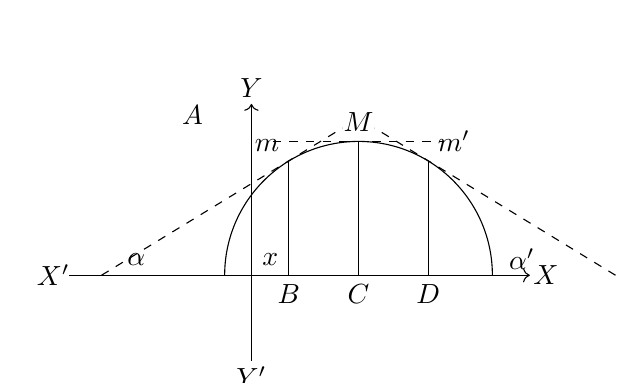
\begin{tikzpicture}[scale=0.68]
  \draw (-0.5,0) arc (180:0:2.5);
  \draw[->] (-3.4,0) -- (5.2,0);
  \node at (5.5,0) {$X$};
  \node at (-3.7,0) {$X'$};
  \draw[->] (0,-1.6) -- (0,3.2);
  \node at (0,3.5) {$Y$};
  \node at (0,-1.9) {$Y'$};
  \draw (0.7,0) -- (0.7,2.135);
  \draw (2,0) -- (2,2.5);
  \draw (3.3,0) -- (3.3,2.135);
  \draw[dashed] (0.4,2.5) -- (3.6,2.5);
  \draw[dashed] (-2.8,0) -- (1.7,2.75);
  \draw[dashed] (6.8,0) -- (2.3,2.75);
  \node at (-1.1,3.0) {$A$};
  \node[above] at (2,2.5) {$M$};
  \node[above left] at (0.7,2.135) {$m$};
  \node[above right] at (3.3,2.135) {$m'$};
  \node[below] at (0.7,0) {$B$};
  \node[below] at (2,0) {$C$};
  \node[below] at (3.3,0) {$D$};
  \node at (-2.15,0.3) {$\alpha$};
  \node at (5.05,0.3) {$\alpha'$};
  \node at (0.35,0.3) {$x$};
\end{tikzpicture}
\qquad
% FIGURE (printed p.64, right "B"): secant O--o (angle v) and tangent at o (angle
% alpha) to a hump curve peaking at P; right triangle legs h (horizontal) and k
% (vertical) with k/h = tg v; O, P, S on the axis, o above P. Redrawn in TikZ.
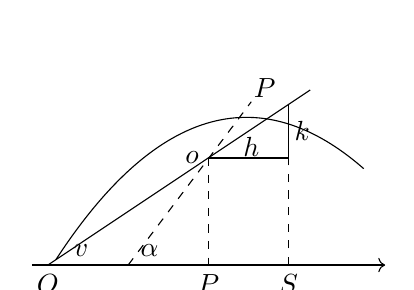
\begin{tikzpicture}[scale=0.68]
  \draw[->] (-0.3,0) -- (6.3,0);
  \draw (0.15,0.1) .. controls (2.3,3.4) and (4.3,3.2) .. (5.9,1.8);
  \draw (0,0) -- (4.9,3.27);
  \draw[dashed] (1.5,0) -- (3.8,3.05);
  \draw[dashed] (3,2) -- (3,0);
  \draw (3,2) -- (4.5,2) -- (4.5,3.0);
  \draw[dashed] (4.5,0) -- (4.5,2);
  \node[above] at (4.05,2.95) {$P$};
  \node[left] at (3,2) {$o$};
  \node at (0.62,0.28) {$v$};
  \node at (1.9,0.28) {$\alpha$};
  \node at (3.8,2.2) {$h$};
  \node at (4.75,2.5) {$k$};
  \node[below] at (0,0) {$O$};
  \node[below] at (3,0) {$P$};
  \node[below] at (4.5,0) {$S$};
\end{tikzpicture}
\end{center}

\begin{center}
$OP = x$;\quad $oP = y$;\quad The point $(x, y) = o$.
\end{center}

But in order to determine the tangent, one must know its relation to the secant.
According to figure B, $\dfrac{k}{h} = \operatorname{tg} v$, and $v$ the angle which
the secant forms with the positive direction of the axis of the $x$'s. As the points
of intersection, $p$ and $o$, move nearer to one another, the secant approaches
becoming ``touching'', and, the
% ---- printed p.65 (PDF 70) ----
moment the points coincide, will be a tangent. Since now
$\dfrac{k}{h} = \operatorname{tg} v$, then $\lim\dfrac{k}{h} = \dfrac{dy}{dx}$ must be
$\operatorname{tg}\alpha$, $\alpha$ being the angle which the tangent to the point
$(x, y)$ forms with the axis of the $x$'s.

From figure A one sees that $\operatorname{tg}\alpha$ passes, at the maximum point,
over from being positive to being negative $= \operatorname{tg}\alpha'$;
$\dfrac{dy}{dx}$ thus changes sign at $M$, and must then at this point be 0.

Since, further,
\[
\frac{d^{2}y}{dx^{2}} = \frac{d\cdot\frac{dy}{dx}}{dx}
= \frac{d\operatorname{tg}\alpha}{dx},
\]
$\dfrac{d^{2}y}{dx^{2}}$ denotes the increment by which $\operatorname{tg}\alpha$
varies when $x$ grows. But $\operatorname{tg}\alpha$ (to the point $m$) is evidently,
when $x$ varies from $B$ to $D$, in constant decrease, so that the increment is
negative; $\dfrac{d^{2}y}{dx^{2}}$ must, then, with respect to the maximum, be
negative, and the formula $\mp\dfrac{1}{r}$ give $-\dfrac{1}{r}$.

In this way, then, each differential coefficient can, in accordance with the
systematic connection of the derived functions, come to play a peculiar role.

\begin{center}
\textbf{3) The Integral.}
\end{center}
\phantomsection
\addcontentsline{toc}{subsection}{3) The Integral}

An analysis of the infinite is necessarily at the same time an analysis of the
finite, just as also every analysis of the negative is at the same time an analysis
of the positive, every analysis of concept likewise an analysis of representation.

In relation to the line as the positive, the point, the limit of the line, is the
negative; when the line is a representation, the point is a thought. In relation to
the surface as the positive, the line, the limit of the surface, is the negative: the
surface
% ---- printed p.66 (PDF 71) ----
is represented when the line is thought. In relation to the body, the positive, the
surface, the limit of the body, is the negative.

In relation to the still undetermined place, the negative, the determinate point is
the positive; indeed, in relation to the mass, the material object, the mathematical
body itself is a negation, an object of thought, a concept.

The infinite and yet withal finite reciprocal determination of negative and positive,
of point and line, of line and surface, of surface and body, which occupies
mathematics, becomes then also recognizable by the categories: discreteness and
continuity.

A line, this given continuum, can be divided, and each part is again a line. Since now
each part becomes the smaller, the greater the number of parts becomes, one concludes
that every line must be able to be divided, or rather: ``be thought as divided into
infinitely many infinitely small parts''.

The inference leads, however, at once into several difficulties. If each smallest part
of the divided line is still a line, a little continuum, then this continuum must
again be able to be divided into infinitely many infinitely small parts.

The smallest part is then so far from being the smallest possible, that on the
contrary it even seems to become equal in size to the whole line, since the part and
the whole both admit of being divided into ``infinitely many infinitely small
parts''. If, on the other hand, each smallest part of the divided line can no longer
be divided, then this smallest part is no more a line but a point.

The divided line then comes to consist in an infinite discreteness of infinitely many
points; but the point is precisely the negation of the line, is, punctually
understood, without any extension, a Not-Line. According to the cited inference the
line came then to consist, not of countless small lines, but of infinitely many
Not-Lines. But to imagine a real, positive line composed of infinitely many Not-Lines
is about as difficult as to imagine
% ---- printed p.67 (PDF 72) ----
a real, positive Thanks composed of infinitely many Un-thanks.

What mathematics really puts into the expression ``infinitely many infinitely small
parts'' cannot, however, be known from turns of phrase; it must show itself in the
deed. If we seek the infinite smallness of the parts in the differential, we must seek
their so-called infinite sum in the integral; from summation and integration we shall
then strive to find out the determination of the integral.

\begin{center}
\textbf{a) Summation.}
\end{center}
\phantomsection
\addcontentsline{toc}{subsubsection}{a) Summation}

If a line $x$ is assumed to be divided into infinitely many infinitely small parts,
and each of these parts --- without its yet being decided whether they are points or
lines --- is denoted by $dx$, then mathematics is incontestably right when it denotes
the whole line by the infinite sum of the parts $\int dx = x$.

But what now is $dx$, point or line? Should dialectics explain itself on this, it
would say: it is not a point, for it is really a line; it is not a line, for it is
essentially a point. It is a line which has just shrunk to a point; a point which is
just in the process of being expanded into a line.

What dialectics thus says in its language is precisely what mathematics presupposes in
its practice. $dx$ is, as already shown, just as little 0 as a finite magnitude. If
$dx$ were 0, then $\int dx$ would simply be $\infty\cdot 0$, but this is by no means
the case. If one sets $\int dx = \infty\cdot 0 = \dfrac{1}{0}\cdot 0 = \dfrac{0}{0}$,
then there is here no difference between the integral and a still undetermined
differential coefficient, whose value can thus be both finite and infinite.

Mathematics, then, does not engage in determining $dx$ immediately, be it as point or
as line;
% ---- printed p.68 (PDF 73) ----
$dx$ is determined only in a relation, as, for example, by $dy$; so that the law of
change can show itself in $f(x) = y$.

In $f(x) = y$ the increment for $x$, the independent, must naturally be constant; for
if $dx$ varied, the changes would have to be subject to a certain law, and $x$ could
then not be independent. As regards the increment for $y$, the dependent, the
differential coefficient $\dfrac{dy}{dx}$ expresses a definite relation, but the
individual $dy$ can, on the other hand, be among themselves either equal or unequal.

\begin{center}
% FIGURE (printed p.68, left): right triangle ABC (right angle at C) with AC = x
% (base) subdivided into equal dx and BC = y (right side) into equal dy; hypotenuse
% AB. All dy equal (straight line). Redrawn in TikZ.
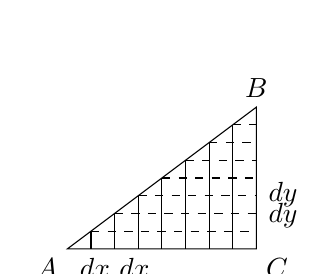
\begin{tikzpicture}[scale=0.6]
  \draw (0,0) -- (4,0) -- (4,3) -- cycle;
  \draw (0.5,0) -- (0.5,0.375);
  \draw (1,0) -- (1,0.75);
  \draw (1.5,0) -- (1.5,1.125);
  \draw (2,0) -- (2,1.5);
  \draw (2.5,0) -- (2.5,1.875);
  \draw (3,0) -- (3,2.25);
  \draw (3.5,0) -- (3.5,2.625);
  \draw[dashed] (0.5,0.375) -- (4,0.375);
  \draw[dashed] (1,0.75) -- (4,0.75);
  \draw[dashed] (1.5,1.125) -- (4,1.125);
  \draw[dashed] (2,1.5) -- (4,1.5);
  \draw[dashed] (2.5,1.875) -- (4,1.875);
  \draw[dashed] (3,2.25) -- (4,2.25);
  \draw[dashed] (3.5,2.625) -- (4,2.625);
  \node[below left] at (0,0) {$A$};
  \node[above] at (4,3) {$B$};
  \node[below right] at (4,0) {$C$};
  \node[below] at (1.0,0) {$dx\ dx$};
  \node[right] at (4.05,1.15) {$dy$};
  \node[right] at (4.05,0.7) {$dy$};
\end{tikzpicture}
\end{center}

\begin{center}
$AC = x$;\quad $BC = y$.
\end{center}

In the triangle $ABC$ one has:
\[
\begin{aligned}
BC &= y = dy + dy + dy + \dots\\
AC &= x = dx + dx + dx + \dots
\end{aligned}
\]
In each of these infinite sums the terms are among themselves equal, namely
$dy = dy$, just as $dx = dx$; but only in a single case, namely when
$\angle BAC = 45^{\circ}$, is $dy = dx$, and the differential quotient
$\dfrac{dy}{dx} = \dfrac{0}{0} = 1$.

In the figures $AA'BC$ and $AA''BC$ one still has, as before, $dx = dx$, but on the
other hand not $dy = dy^{1}$. If the dependence in which $y$ stands to $x$ is viewed,
for one case by the curve $AA'B$, for another by the curve $AA''B$; then it is evident
from this that the individual $dy$ in the infinite sum:
\[
y = dy + dy' + dy'' + dy''' + \dots
\]

\begin{center}
% FIGURE (printed p.68, right): two curves AA'B (lower) and AA''B (upper) from A to
% B over base AC = x, right side BC = y; the staircase of equal dx but unequal dy
% under the lower curve. Redrawn in TikZ.
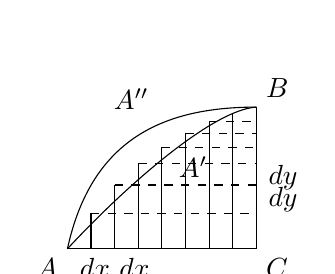
\begin{tikzpicture}[scale=0.6]
  \draw (0,0) -- (4,0) -- (4,3);
  \draw (0,0) .. controls (1.3,1.4) and (3.1,2.95) .. (4,3);
  \draw (0,0) .. controls (0.5,2.3) and (2,3) .. (4,3);
  \draw (0.5,0) -- (0.5,0.75);
  \draw (1,0) -- (1,1.35);
  \draw (1.5,0) -- (1.5,1.8);
  \draw (2,0) -- (2,2.15);
  \draw (2.5,0) -- (2.5,2.45);
  \draw (3,0) -- (3,2.7);
  \draw (3.5,0) -- (3.5,2.88);
  \draw[dashed] (0.5,0.75) -- (4,0.75);
  \draw[dashed] (1,1.35) -- (4,1.35);
  \draw[dashed] (1.5,1.8) -- (4,1.8);
  \draw[dashed] (2,2.15) -- (4,2.15);
  \draw[dashed] (2.5,2.45) -- (4,2.45);
  \draw[dashed] (3,2.7) -- (4,2.7);
  \node[below left] at (0,0) {$A$};
  \node[above right] at (4,3) {$B$};
  \node[below right] at (4,0) {$C$};
  \node[above] at (1.35,2.75) {$A''$};
  \node[below right] at (2.15,2.15) {$A'$};
  \node[below] at (1.0,0) {$dx\ dx$};
  \node[right] at (4.05,1.5) {$dy$};
  \node[right] at (4.05,1.05) {$dy$};
\end{tikzpicture}
\end{center}

\begin{center}
$AC = x$;\quad $BC = y$.
\end{center}

will not only be, in both cases, among themselves unequal, but
% ---- printed p.69 (PDF 74) ----
the inequality withal also different for every one of the different cases.

If one now holds fast the presupposition that every mathematical point must, as
negation of all magnitude, be 0, so that $0 = 0$ in this case is as Nothing $=$
Nothing; then it is clear that $dx$ in the line $x$ can just as little be a
mathematical point as $dy$ in the line $y$, for from Nothing comes Nothing, and
between Nothing and Nothing there is no relation. But that $dx$ and $dy$ are
nevertheless not restricted to being lines of finite extension is seen also from
this, that the law of dependence for $y$ with respect to $x$ is each time so
determined that the relation $\dfrac{dy}{dx}$ is preserved even in $\dfrac{0}{0}$.

If the differential denotes a moment in the infinite discreteness of the line, then
the integral denotes the merging of the discrete moments into the finite continuum;
if the differential denotes the infinitely small term, then the integral denotes the
infinitely great sum. If the infinitely small term, be it $dx$ or $dy$, cannot be
directly stated, then the infinite summation, the summation of the countless terms,
cannot be directly carried out either.

If one presupposes $f(a + dx) - f(a) = f'(a)\,dx$, one obtains, by constantly adding
$dx$,
\[
\begin{array}{r@{\;=\;}l}
f(a+2dx) - f(a+dx) & f'(a+dx)\,dx,\\[2pt]
f(a+3dx) - f(a+2dx) & f'(a+2dx)\,dx,\\[2pt]
\hdotsfor{2}\\[2pt]
f(a+ndx) - f(a+(n-1)dx) & f'(a+(n-1)dx)\,dx\\[2pt]
\hline
\end{array}
\]
and by addition:
\[
f(a+ndx) - f(a) = f'(a)\,dx + \dots f'(a+(n-1)dx)\,dx.
\]

If $dx$ is infinitely small, $f'(a)\,dx$, $f'(a+dx)\,dx \dots$ likewise, one must set
$n = \infty$, in order that $ndx$ may become a finite magnitude, and $a + ndx$ in
$f(a + ndx)$ is set $= b$.

But when the matter is thus conceived, the old difficulties return; it is only by a
leap that one can here reach from $n$ to $\infty$, and when one has then --- naturally
by leaping over infinitely many terms --- made this leap,
% ---- printed p.70 (PDF 75) ----
the sum, $\infty\, dx$, is still so indeterminate a magnitude that it can be set
$= x$, $= \dfrac{1}{2}x = 1000\,x$, $= \dfrac{1}{1000}x$, and so on.

A sum is, according to its concept, a number, a finite number. An infinite number, an
infinite sum, a summation of an infinite number are at bottom nothing but
contradictions. If an infinite summation is to be carried out, the task must be solved
either by approach, thus in approximateness, or by a transformation.

\begin{center}
\textbf{b) Integration.}
\end{center}
\phantomsection
\addcontentsline{toc}{subsubsection}{b) Integration}

In the series $1 + \dfrac{1}{2} + \left(\dfrac{1}{2}\right)^{2}
+ \left(\dfrac{1}{2}\right)^{3} + \dots$ the number of terms is infinite. A summation
of these terms can now, in the first place, take place by approach, in that, with
regard to the convergence of the series, one takes as many terms as the accuracy of
the calculation requires; but without losing oneself in a counting-together of
countless terms, one could also by another way attain a result, and even an exact
result, namely by finding the quotient from which the infinite series springs.
Instead of an infinite summation, a law-governed reduction is then employed: the task
is solved by being transformed.

A telling example of the transformation of tasks we have in the treatment of the
relation of broken lines to curves.

At the transition from finite to infinite, mathematics begins with the assumption
that the circle is a polygon of an infinite number of infinitely small sides. How
this proposition is applied in elementary geometry is well known; in the higher
analysis the matter can be presented thus:

\begin{center}
% FIGURE (printed p.70): a circular arc (m ... C ... B ... n) with its chord a = CB;
% the triangle BCD (apex D to the right), b = CD, c = BD, and the dashed altitude
% D--e to the chord. Illustrates the projection a = b cos C + c cos B. Redrawn in
% TikZ.
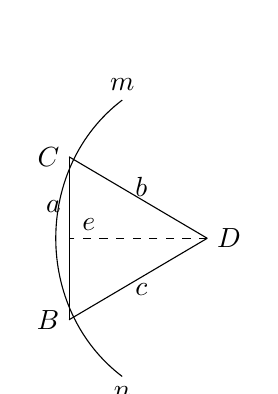
\begin{tikzpicture}[scale=0.9]
  \draw (0.35,1.95) .. controls (-0.9,1.0) and (-0.9,-1.0) .. (0.35,-1.95);
  \coordinate (Cc) at (-0.4,1.15);
  \coordinate (Bb) at (-0.4,-1.15);
  \coordinate (Dd) at (1.55,0);
  \coordinate (Ee) at (-0.4,0);
  \draw (Cc) -- (Bb);
  \draw (Cc) -- (Dd);
  \draw (Bb) -- (Dd);
  \draw[dashed] (Dd) -- (Ee);
  \node[above] at (0.35,1.95) {$m$};
  \node[below] at (0.35,-1.95) {$n$};
  \node[left] at (Cc) {$C$};
  \node[left] at (Bb) {$B$};
  \node[right] at (Dd) {$D$};
  \node at (-0.62,0.45) {$a$};
  \node at (-0.12,0.2) {$e$};
  \node at (0.62,0.72) {$b$};
  \node at (0.62,-0.72) {$c$};
\end{tikzpicture}
\end{center}

$a = b\cos C + c\cos B$, according to the figure; but
\[
\cos C = 1 - \frac{C^{2}}{1\cdot2} + \frac{C^{4}}{1\cdot2\cdot3\cdot4} \dots,
\]
and
\[
\cos B = 1 - \frac{B^{2}}{1\cdot2} + \frac{B^{4}}{1\cdot2\cdot3\cdot4} \dots
\]
% ---- printed p.71 (PDF 76) ----
Thus
\[
\begin{aligned}
a &= b\left(1 - \frac{C^{2}}{1\cdot2} \dots\right)
+ c\left(1 - \frac{B^{2}}{1\cdot2} \dots\right)
= b - \frac{bC^{2}}{1\cdot2}\dots\\
&\quad {}+ c - \frac{cB^{2}}{1\cdot2}\dots
= b + c - \frac{bC^{2}}{1\cdot2}\dots - \frac{cB^{2}}{1\cdot2}\dots
\end{aligned}
\]

The fundamental question is what, according to the stated law of change, will happen
when the terms become infinitely small; and the answer is that $\dfrac{bC^{2}}{1\cdot2}$
and $\dfrac{cB^{2}}{1\cdot2}$, the terms of the second order, will vanish, and leave
$a = b + c$.

In the finite sense the arc $CB$ corresponding to $a$ as chord is $< b + c$, but
$> a$; but, since $a = b + c$, the whole $BCD$ has shrunk to a point, which is
nevertheless not a point, but an element in a line.

The line in which $BCD$ is an element is not a polygon-side, but a circle-periphery.
In so far as there is here in $a$ still the least remnant of a polygon-side, $BCD$ is
not an element in a line, but a real triangle; the triangle $BCD$ can vanish, but only
in the curved line.

Instead of proving either that the circle is a polygon or the polygon a circle,
mathematics has on the contrary transformed the task, and proved that a circle is
essentially different from a polygon, and a polygon from a circle.

The view that a curved line is at bottom a broken line is intimately connected with
the conception that integration is a summation. Instead of conceiving integration as
an infinite summation, we must rather regard it as a transformation of the task of
summation, more closely determined by the express opposition to
differentiation\footnote{``Integration is the inverse calculation of differentiation.
It consists, when a differential is given, in determining the function of which it is
the differential, and in general, when a differential equation is given, in
determining its corresponding primitive equation''. Ramus.\ Differ.\ Integr.\ S.\ 34.
That the higher theories of the summation of infinite series rest on reductions and
transformations is evident. A series such as the Eulerian:
$x^{-a_{m}-1}\int_{0}^{x} s_{n,m}\,x^{a_{m}}\,dx = s_{n,m-1}$. (Ramus.\ Diff.\
Intgr.\ S.\ 308) admits, naturally, still less of being treated by direct summation
than, for example, the series:
$1 + \frac{1}{2} + \left(\frac{1}{2}\right)^{2} + \dots$}.
% ---- printed p.72 (PDF 77) ----
Leibnitz, who discovered differentiation, as the direct tangent method, found in
integration the inverse tangent method.

With respect to the circle, $y = f(x) = \pm\sqrt{2rx - x^{2}}$ was in the foregoing
given as the original function; the task was then to find the derived functions,
namely $\dfrac{dy}{dx} = \dfrac{r - x}{\sqrt{2rx - x^{2}}}$, and thereby to determine
the angle which the tangent to a point in the circle will form with the positive
direction of the axis of abscissas. By inserting different values for $x$ one
determines the tangent for the different points in the curve.

If we choose the ellipse, and place the origin of the coordinates at the centre, then
we again have $y = f(x)$, but this time determined as
$\dfrac{b}{a}\sqrt{a^{2} - x^{2}}$.

\begin{center}
% FIGURE (printed p.72): ellipse centred at C, semi-axes CD = a (horizontal, right
% vertex D) and CE = b (vertical, bottom vertex E); a point B on the ellipse (upper
% right) with coordinates x (horizontal from C) and y (vertical), and its reflection
% B'; top-left point A. Redrawn in TikZ.
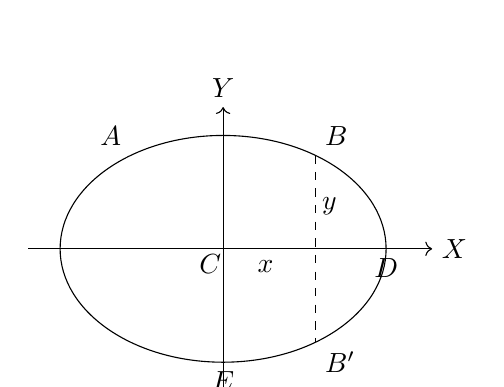
\begin{tikzpicture}[scale=0.9]
  \draw (0,0) ellipse (2.3 and 1.6);
  \draw[->] (-2.75,0) -- (2.95,0);
  \node[right] at (2.95,0) {$X$};
  \draw[->] (0,-2.0) -- (0,2.0);
  \node[above] at (0,2.0) {$Y$};
  \draw[dashed] (1.3,1.32) -- (1.3,-1.32);
  \node at (-0.18,-0.22) {$C$};
  \node[below] at (2.3,0) {$D$};
  \node[below] at (0,-1.6) {$E$};
  \node[above left] at (-1.3,1.32) {$A$};
  \node[above right] at (1.3,1.32) {$B$};
  \node[below right] at (1.3,-1.32) {$B'$};
  \node at (0.6,-0.25) {$x$};
  \node at (1.5,0.6) {$y$};
\end{tikzpicture}
\end{center}
\begin{center}
$CD = a$;\quad $CE = b$.
\end{center}

The first differential coefficient corresponding to this is then found to be
$-\dfrac{b}{a}\dfrac{x}{\sqrt{a^{2}-x^{2}}}$, whereby likewise the direction of the
tangent for every point in the ellipse can be determined. If, for example, $x = 0$,
one gets the direction of the tangent at the end-point of the minor axis; for then
\[
\frac{dy}{dx} = -\,\frac{b}{a}\,\frac{0}{\sqrt{a^{2}-0}} = 0.
\]
If $x = a$, one gets the tangent to the end-point of the major axis, namely
\[
\frac{dy}{dx} = -\,\frac{b}{a}\,\frac{a}{\sqrt{a^{2}-a^{2}}}
  = -\,\frac{ba}{\sqrt{0}} = -\,\frac{ba}{0} = \infty.\footnotemark
\]
\footnotetext{To AB, the tangent, which forms an angle $= 0$ with the axis of the
$x$'s, there corresponds a tangent (in numerical value) $= 0$; to $A'B'$, a tangent
which forms an angle with the axis of the $x$'s $= 90^{\circ}$, there corresponds a
tangent $= \infty$.}
In both these cases, then, the original function $f(x)$ was given, and the task was to
find the derived one,
\[
\frac{dy}{dx} = \frac{d\,f(x)}{dx}.
\]
These, then, were examples of the direct tangent method.

But now, conversely, a derived function $f'(x) = \dfrac{dy}{dx}$ could also be given,
and the task become to find the corresponding original one, $f(x) = y$.

1)~Example. There is given an equation
$\dfrac{dy}{dx} = \dfrac{r-x}{\sqrt{2rx-x^{2}}} = f'(x)$, whereby a curve's tangent is
determined; the task
% flag: the following display interrupts the sentence in the print --
% "Opgaven" (p.73) ... [display] ... "er, at finde" (p.74 top)
\[
\text{A series such as }\int_{0}^{x} 2x\,dx
  = \mathrm{Lim}\,2\frac{x^{2}}{n^{2}}\,(1+2+3+4+\cdots (n-1))
\]
is not summed, but reduced:
\[
= \mathrm{Lim}\,2\frac{x^{2}}{n^{2}}\left(\frac{(n-1)\,n}{2}\right)
= \mathrm{Lim}\,x^{2}\,\frac{n-1}{n}
= \mathrm{Lim}\,x^{2}\left(1-\frac{1}{n}\right).
\]
From the result of the reductions it emerges that the sum of the series, when one
sets $n = \infty$, will give $x^{2}$, and that one thus obtains
$\int_{0}^{x} 2\,x\,dx = x^{2}$; but such a summation is no longer summation: the
limit is transgressed, the task transformed.
is, to find the curve's original equation: $f(x) = y$. By integration, the inverse
tangent method, one then finds
\[
\int f'(x)\,dx = f(x) = \pm\sqrt{2rx-x^{2}};
\]
i.e. one finds that the curve in question is a circle.

2)~Example. There is given an equation
$\dfrac{dy}{dx} = -\,\dfrac{b}{a}\dfrac{x}{\sqrt{a^{2}-x^{2}}}$, whereby the tangent
for a curve is determined; one is now, by integration, the inverse tangent method, to
find what kind of curve it is, and then finds
$\int f'(x)\,dx = \dfrac{b}{a}\sqrt{a^{2}-x^{2}} = f(x)$, which shows that the curve is
an ellipse.

The opposition between integration and differentiation can, with respect to powers,
be made intuitive thus: by differentiation one passes from $f(x) = x^{n}$ to
$f'(x) = nx^{n-1}$; by integration one passes conversely from
$f'(x)\,dx = nx^{n-1}\,dx$ to $f(x) = x^{n}$: by differentiation one has
$d(x^{n}) = n\,x^{n-1}\,dx$, by integration one obtains
$\int n\,x^{n-1}\,dx = \int d(x^{n}) = x^{n}$; one differentiates a power by
multiplying by the exponent and subtracting 1 from the exponent; one integrates a
power by adding 1 to the exponent and dividing by the increased exponent.
\[
x^{n} = \int n\,x^{n-1}\,dx = n\int x^{n-1}\,dx, \quad\text{thus:}\quad
\frac{x^{n}}{n} = \int x^{n-1}
\]
% flag: the print breaks this display mid-expression -- it ends at
% "= \int x^{n-1}" and the orphaned "dx" starts the next text line
$dx$, if one now sets $n-1 = m$, $n = m+1$, then one has:
\[
\int x^{m}\,dx = \frac{x^{m+1}}{m+1} + C.
\]
But what now does $C$, the arbitrary constant, mean?

\begin{center}\textbf{c)~The Determination of the Integral.}\footnotemark\end{center}
\phantomsection
\addcontentsline{toc}{subsubsection}{c) The Determination of the Integral}
\footnotetext{``There is no general method for finding
$\int X\,dx$ expressed under finite form, when $X$ is an explicit
function of $x$ under finite form, whereas $\dfrac{dX}{dx}$
can always be expressed under finite form. For integration is an inverse
calculation, and therefore generally leads to new functions''\dots\
``Just as subtraction, division, root-extraction, which are inverse
calculations of addition, multiplication, raising to a power, have led
to new magnitudes: negative, fractional, rational, and imaginary.''
Ramus. Differential- og Integral-Rgn. S.\,36.

That integration, moreover, is on the whole determined by its principled
opposition to differentiation lies in the nature of the matter, and is seen from
manifold forms. Since a constant can have no differential, it
can have no integral either. When $a$ is constant,
$\int a\,X\,dx = a\int X\,dx$. If $d(\sin x) = \cos x\,dx$, then
$\int \cos x\,dx = \int d(\sin x) = \sin x$; if
$d(\cos x) = -\sin x\,dx$, then
$\int -\sin x\,dx = \int d(\cos x) = \cos x$, and
$-\cos x = \int \sin x\,dx$; if
$d(f(x) \pm \Phi(x)) = f'(x)\,dx \pm \Phi'(x)\,dx$, then
$\int (f'(x)\,dx \pm \Phi'(x)\,dx) = \int d(f(x) \pm \Phi(x))
= f(x) \pm \Phi(x)$; if
$d(f(x)\,.\,\Phi(x)) = f(x)\,d\Phi(x) + \Phi(x)\,df(x)$, and
$f(x)\,d\Phi(x) = d(f(x)\Phi(x)) - \Phi(x)\,df(x)$, then
$\int d(f(x)\,.\,\Phi(x)) = f(x)\Phi(x) = \int f(x)\,d\Phi(x)
+ \int \Phi(x)\,df(x)$, and
$\int f(x)\,d\Phi(x) = f(x)\Phi(x) - \int \Phi(x)\,df(x)$. But in
the further development the matter becomes complicated; already
$\int \dfrac{f(x)}{\Phi(x)}$ requires more elaborate operations:
% flag: print's first term below reads „x α₁" with NO minus sign
% (cf. the „x−α₂" second term); preserved as printed -- likely a typo
% for x−α₁.
\[
\frac{f(x)}{\Phi(x)} = F(x) + \frac{k_1}{x\,\alpha_1}
  + \frac{k_2}{x-\alpha_2}.
\]
Set
\[
\frac{1}{x^2-7x+12} = \frac{1}{(x-4)(x-3)}
  = \frac{k_1}{x-4} + \frac{k_2}{x-3};
  = \frac{k_1\,(x-3) + k_2\,(x-4)}{(x-4)(x-3)};
\]
thus $1 = (k_1 + k_2)\,x - (3k_1 + 4k_2)$. By comparing the
powers of $x$ on both sides it is seen that $k_1 + k_2 = 0$, and
$-3k_1 - 4k_2 = 1$; $4k_1 + 4k_2 = 0$; $k_1 = 1$; $k_2 = -1$.
Consequently:
\[
\frac{1}{x^2-7x+12} = \frac{1}{x-4} - \frac{1}{x-3};
\]
that is:
\[
\int \frac{dx}{x^2-7x+12} = \int \frac{dx}{x-4} - \int \frac{dx}{x-3}.
\]
For $\Phi(x) = (x-\alpha_1)(x-\alpha_2)\dots(x-\alpha_p)^n\,
(x-\alpha)^m\dots$ one has
\[
\int \frac{1\,.\,dx}{x-4},\qquad \int \frac{3\,dx}{(x-4)^2},\qquad
\int \frac{A\,dx}{(x-\alpha)^m}.
\]
Ifr. Ramus. Diffr. Integrl. S.\,37.}
In opposition to the differential as the negative, the integral is the
positive. If the differential is a point, then the integral is a line; if the
differential is a line, then the integral is a surface; if the
differential is a surface, then the integral is a body.

The negative cannot, however, of itself produce the positive,
just as little as the immediately positive can produce the negative:
the transition from negative to positive, and conversely, presupposes a
positing and negating activity, a principle.

In the negating activity the positive is presupposed; it is the
positive that in the negation is, so to speak, cut through, cut across,
or cut off by the negative: the positive is divided. In the positing
activity, conversely, the negative is presupposed. It is not the
being, the positive, that is posited, for the being already is, the
positive is already posited; no, it is precisely the Not-Being, that which
is not yet, the negative, that is posited, and transposed. That the point, the
negative, is posited positively means, in other words, that the beginning of
a line is posited; as the posited beginning is continued, the line
comes to be: the continuation is a movement.

That in this connection the categories division and
composition do not suffice, but that division and movement ought to be opposed to
one another, can be seen from a comparison between the broken and the curved line.

For the broken line a composition holds, for its parts are
finite; it is a piecework which in each and all belongs to finitude.
For the curved line no finite composition whatever holds,
not even the very finest piecing-together; it owes its coming-into-being to
the movement alone, for it belongs to infinity.

The so-called composite movement is not a piecing-together of two
movements, but a movement mediated through two moments.
In so far as there is here the least trace of real piecing-together, the
moved body will change its direction only at finite intervals: there will
arise a broken, not a curved line.

The principle of movement which produces the curved line is intimately
akin to the nature of the function; here is continuity in infinite
discreteness, an invariable in infinite change.

But on the function both the differential and the integral depend.

\begin{center}
% FIGURE (printed p.77): the differential triangle on a curve arc.
% Right angle at C; vertical leg $CA = dy$, horizontal leg $CB = dx$,
% hypotenuse (arc-chord) $AB = ds$; the curve passes through A and B.
% Caption: „A = ds, den uendelig lille Sector."
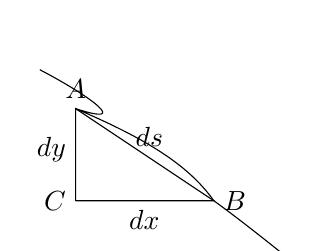
\begin{tikzpicture}[scale=1.3]
  \coordinate (C) at (0,0);
  \coordinate (A) at (0,0.9);
  \coordinate (B) at (1.35,0);
  \draw (C) -- (A) -- (B) -- (C);
  \draw (-0.35,1.28) .. controls (0.15,1.02) and (0.55,0.72) ..
        (A) .. controls (0.7,0.6) and (1.1,0.35) .. (B)
        .. controls (1.6,-0.18) and (1.9,-0.42) .. (2.15,-0.62);
  \node[above] at (A) {$A$};
  \node[left] at (C) {$C$};
  \node[right] at (B) {$B$};
  \node[left] at (0,0.5) {$dy$};
  \node[below] at (0.67,0) {$dx$};
  \node at (0.72,0.62) {$ds$};
\end{tikzpicture}

$A = ds$, the infinitely small sector.
\end{center}

For any curve whatever one has
\[
ds^{2} = dx^{2} + dy^{2}; \quad
ds^{2} = dx^{2}\left(1 + \frac{dy^{2}}{dx^{2}}\right); \quad
\frac{ds}{dx} = \sqrt{1 + \left(\frac{dy}{dx}\right)^{2}}.
\]
This relation is each time peculiarly determined by the curve's
equation; $f(x) = y = \sqrt{a^{2}-x^{2}}$ for the circle;
$\dfrac{b}{a}\sqrt{a^{2}-x^{2}}$ for the ellipse;
$\dfrac{b}{a}\sqrt{x^{2}-a^{2}}$ for the hyperbola;
% flag: print reads „√x √.p" -- a dot set under the second radical
% before p; the parabola is $y=\sqrt{px}=\sqrt{x}\sqrt{p}$, so the dot
% is the multiplication sign, oddly typeset inside the radical.
$\sqrt{x}\,\sqrt{.\,p}$ for the parabola\footnotemark, o.\,s.\,v.
\footnotetext{Ifr. Ramus. Analytisk Geometrie. S.\,13--23.}

What is here indicated by the differential coefficient is, then, not an
already existing fragment, but a moment which has significance
only in relation to the definite law of movement, and the movement therewith either
already entered upon or at least entering.

If the expression
$-\dfrac{b}{a}\dfrac{x}{\sqrt{a^{2}-x^{2}}} = \dfrac{dx}{dy}$ for
the ellipse is inserted, one obtains by reduction
\[
\frac{ds}{dx} = \sqrt{\frac{a^{4} + (b^{2}-a^{2})\,x^{2}}
  {a^{2}(a^{2}-x^{2})}},
\]
% ---- printed p.78 (PDF 83) ----
thus
\[
ds = dx\,\sqrt{\frac{a^{4} + (b^{2}-a^{2})\,x^{2}}{a^{4}-a^{2}x^{2}}},
\]
a formula which is especially used to rectify the ellipse, or
to present it by quadrature\footnotemark, in that by integrating
one obtains:
\[
s = \int_{0}^{x=a} dx\,\sqrt{\frac{a^{4} + (b^{2}-a^{2})\,x^{2}}
  {a^{4}-a^{2}x^{2}}},
\]
a transformation which cannot possibly be brought about by piecing-together, but
is due solely to the movement and the law holding for the movement.
\footnotetext{Every differential equation which has been solved
in such a way that the one variable has been expressed by an integral which
contains the other alone is said to be presented by quadrature.
On quadrature and rectification cf. Ramus. Analytisk Geometrie.
S.\,112--125.}

Even as regards the incommensurable, there can here be no talk of
inexactness, but only of an inner endowment for infinite advance,
infinite development, infinite movement.

From division and movement, then, the opposition between the
differential and the integral in calculations of areas and volumes is thus
understood.

That a surface can be divided into infinitely many infinitely small surfaces, is
incontestable; but that a finite surface cannot be pieced together from
infinitely many infinitely small surfaces, is also incontestable.
Let $\int y\,dx = A$ be the typical formula for any area whatever,
$y = f'(x)$.

1)~Example. In the rectangle $yx$, $y = a$, $ydx = adx$. According to the
formula:
\[
\int y\,dx = \int a\,dx = adx + adx + adx + \dots
\]
\begin{center}
% FIGURE (printed p.78): rectangle; corners B (top-left), C (top-right),
% A (bottom-left), D (bottom-right). Base $AD = x$, right side $DC = y$,
% left side $AB = a$ (so $y = a$, the constant height).
\begin{tikzpicture}[scale=1.0]
  \draw (0,0) rectangle (2.4,1.3);
  \node[below left] at (0,0) {$A$};
  \node[below right] at (2.4,0) {$D$};
  \node[above right] at (2.4,1.3) {$C$};
  \node[above left] at (0,1.3) {$B$};
\end{tikzpicture}

$AD = x$;\quad $DC = y$. \\
$AB = a$.
\end{center}

% ---- printed p.79 (PDF 84) ----
one might almost suppose that mathematics really intended to
count together the countless $adx$, and to piece the finite rectangle together
of infinitely many infinitely small rectangles. This is, however, a
misunderstanding. The task is transformed by being solved. In
$\int y\,dx = \int a\,dx$, $a = y$ is constant; thus
$\int a\,dx = a\int dx = ax$: the rectangle $=$ base $\times$ height.

The solution of the task here by no means aims at showing how
the finite is pieced together from the infinite, but at finding the finite
corresponding to the infinite, namely the $yx$ which admits of being divided into
the countless $ydx$. Should the presentation show how $yx$
arises from $ydx$, then it would have to demonstrate the movement expressly.

2)~Example. In the triangle $ABC$ one has
$\int y\,dx = ydx + y'dx + y''dx + \dots$; but instead of
piecing the triangle together of infinitely many infinitely small rectangles,
mathematics conceives $y$ as a function of $x$;
$y = \operatorname{tg}\alpha\,x$, thus
$ydx = \operatorname{tg}\alpha\,x\,dx$, and this conception corresponds precisely to
the movement.

\begin{center}
% FIGURE (printed p.79): right triangle; A (bottom-left, angle α),
% C (bottom-right), B (top-right). Base $AC = x$, right side $CB = y$;
% straight hypotenuse A--B (the linear function $y=\operatorname{tg}\alpha\,x$)
% with inscribed step-rectangles (the Riemann sum).
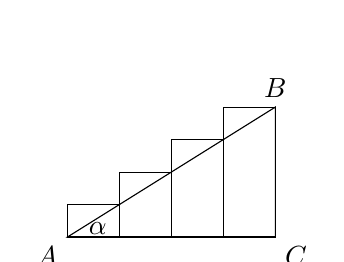
\begin{tikzpicture}[scale=1.1]
  \coordinate (A) at (0,0);
  \coordinate (C) at (2.4,0);
  \coordinate (B) at (2.4,1.5);
  \draw (0,0) rectangle (0.6,0.375);
  \draw (0.6,0) rectangle (1.2,0.75);
  \draw (1.2,0) rectangle (1.8,1.125);
  \draw (1.8,0) rectangle (2.4,1.5);
  \draw (A) -- (C) -- (B) -- cycle;
  \node[below left] at (A) {$A$};
  \node[below right] at (C) {$C$};
  \node[above] at (B) {$B$};
  \node at (0.35,0.1) {$\alpha$};
\end{tikzpicture}

$AC = x$;\quad $CB = y$.
\end{center}

One thus obtains
$\int y\,dx = \int \operatorname{tg}\alpha\,x\,dx
= \operatorname{tg}\alpha\int x\,dx$; but according to the law stated for the
integration of a power, $\int x\,dx = \dfrac{x^{2}}{2}$, and thus
\[
\operatorname{tg}\alpha\int x\,dx = \operatorname{tg}\alpha\,
\frac{x^{2}}{2} = \operatorname{tg}\alpha\,x\,\frac{x}{2}
= y\,\frac{x}{2}:
\]
the area of the triangle $=$ base $\times\ \tfrac{1}{2}$ height.

\begin{center}
% FIGURE (printed p.80): parabola $y^2=px$ with vertex at A. Rectangle
% D (top-left), B (top-right), E (bottom-right), A (bottom-left, = vertex);
% upper branch A--C--B, lower branch A--H (below the base); chord A--B;
% dashed vertical G (on chord) -- F (on base) -- H (on lower branch).
% Labels: $AE=x$, $EB=y$, $GFH=p$. Schematic redraw.
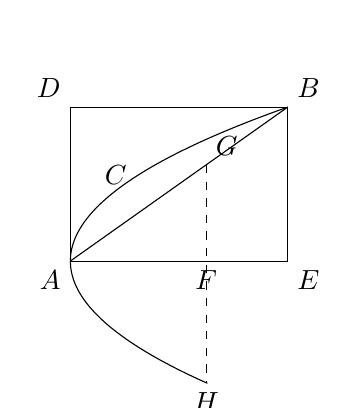
\begin{tikzpicture}[scale=1.15]
  \coordinate (A) at (0,0);
  \coordinate (E) at (2.4,0);
  \coordinate (B) at (2.4,1.7);
  \coordinate (D) at (0,1.7);
  \draw (D) -- (B) -- (E) -- (A) -- (D);
  \draw (A) -- (B);
  \draw[domain=0:1.7,smooth,variable=\t] plot ({(\t*\t)/1.204},{\t});
  \draw[domain=-1.35:0,smooth,variable=\t] plot ({(\t*\t)/1.204},{\t});
  \draw[dashed] (1.5,1.06) -- (1.5,-1.35);
  \node[above left] at (D) {$D$};
  \node[above right] at (B) {$B$};
  \node[below right] at (E) {$E$};
  \node[below left] at (A) {$A$};
  \node[below] at (1.5,0) {$F$};
  \node[above right] at (1.5,1.06) {$G$};
  \node[below] at (1.5,-1.35) {$H$};
  \node at (0.5,0.95) {$C$};
\end{tikzpicture}

$AE = x$;\quad $EB = y$. \\
$GFH = p$.
\end{center}

For a parabola, whose equation, $y^{2} = px$, shows
$y = f'(x) = \sqrt{p}\,\sqrt{x}$,
\[
\int y\,dx = \sqrt{p}\int \sqrt{x}\cdot dx = \sqrt{p}\int x^{\frac12}\,dx
  = \sqrt{p}\,\frac{x^{\frac{3}{2}}}{\frac{3}{2}}
  = \frac{2}{3}\sqrt{p}\,x^{\frac12}\cdot x = \frac{2yx}{3}.
\]
\[
\text{The segment } ACB = \frac{2yx}{3} - \frac{yx}{2}
  = \left(\frac{4}{6} - \frac{3}{6}\right)xy = \frac{1}{6}xy.
\]
\[
\text{The area } ADBCA = xy - \frac{2}{3}xy = \frac{1}{3}xy
  = 2\times \text{the segment } ACB.\text{\footnotemark}
\]
\footnotetext{We have found the area $ABCE = \dfrac{2}{3}xy = \dfrac{2}{3}$
of a rectangle, which can be reduced to a square; the parabola can therefore,
what the other conic sections cannot, be squared under finite
form.}
In all such cases that which has come to be is treated not as an immediate
being, but according to its coming-into-being; the function expresses the law of
the coming-into-being.

The coming-into-being here too presupposes something already come-to-be. In that
integration, on the presupposition of the movement expressed in the changes,
leads the infinite back to finite determinacy, the definite integral must
be stated by an added constant. The constant is precisely
the limit in which the finite touches the infinite in the
movement\footnote{The doctrine of the constant must not be misunderstood, as if
mathematics, in order to indicate definite relations and express the definite
laws, necessarily had to have individual invariable terms; on the contrary,
the deeper one penetrates into the higher analysis --- into differentials with
several independents (Ramus. Diff. Intgr. S.\,149 and following), into the
generation of curves and surfaces (Ramus. Analytisk Geometrie. S.\,135 and
following), into the contact, osculation, evolution of lines, and so forth --- the
more evident it becomes that every term of relation is infinitely variable, and only
the system of laws the essential, the constant, the eternal. In so far as
materialism, with respect to the relations exact in mechanical and chemical
attractions, would infer from the constancy of the relations to the invariability of
the fundamental parts by appealing to the mathematical, the inference is false.}.

% ---- printed p.81 (PDF 86) ----
Example. From rational mechanics the relation between the velocity
$v = \dfrac{dx}{dt}$, and the moving force
$\varphi = \dfrac{d^{2}x}{dt^{2}}$, has already been brought out.

If now 1) the velocity is constant, then one sets $\dfrac{dx}{dt} = a$, where
$a$ is the constant. From $dx = adt$ one then gets by integration
$\int dx = \int adt = a\int dt$, or: $x = at + b$; $b$ is an
added arbitrary constant, for if one differentiates $x = at + b$,
one obtains again $dx = d\cdot at + db = adt + 0$. The meaning of the
added constant is then elucidated thus: for $t = 0$, $x = b$, thus
$b$ is the distance of the mass from the point of departure at the beginning of the
movement.

If 2) the force $\varphi$ is constant, $= k$, one has
$\dfrac{d^{2}x}{dt^{2}} = k$, and $\dfrac{d^{2}x}{dt} = kdt$, which,
integrated, gives $\dfrac{dx}{dt} = \int kdt$; thus
$\dfrac{dx}{dt} = kt + c$, and $c$, the constant, an initial velocity,
for, when $t = 0$, $\dfrac{dx}{dt} = c$. Integrating again, one obtains
\[
\int dx = \int (kt + c)\,dt = \int (ktdt + cdt)
  = k\int t\,dt + c\int dt,
\]
thus: $x = \dfrac{1}{2}kt^{2} + ct + d$, where $d$ is a new constant,
and so forth.

The meaning of the constant shines forth likewise from the calculation of area.

% ---- printed p.82 (PDF 87) ----
If one determines the area of the triangle by the formula $y\dfrac{x}{2}$ from
the standpoint of finitude, then from the standpoint of infinity one must
apply the formula $\int y\,dx = \dfrac{xy}{2} + C$. Here it is presupposed
that $x$, the independent, and $y$, the dependent, vary to
infinity: the added constant points to the movement.

\begin{center}
% FIGURE (printed p.82): right triangle $O$ (bottom-left, origin),
% $D$ (bottom-right), $B$ (top-right); hypotenuse $O$--$B$; point $b$ on
% the hypotenuse above $d$ on the base; inscribed Riemann strips between
% $d$ and $D$. Labels: $OD=x$, $BD=y$, $Od=x'=bd=y'$. Schematic redraw.
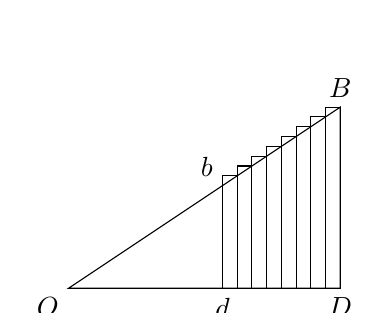
\begin{tikzpicture}[scale=1.15]
  \coordinate (O) at (0,0);
  \coordinate (D) at (3,0);
  \coordinate (B) at (3,2);
  \foreach \i in {0,...,7}{
    \pgfmathsetmacro\xa{1.7+\i*0.1625}
    \pgfmathsetmacro\xb{\xa+0.1625}
    \pgfmathsetmacro\hh{(2/3)*\xb}
    \draw (\xa,0) rectangle (\xb,\hh);
  }
  \draw (O) -- (D) -- (B) -- cycle;
  \node[below left] at (O) {$O$};
  \node[below] at (3,0) {$D$};
  \node[above] at (B) {$B$};
  \node[below] at (1.7,0) {$d$};
  \node[above left] at (1.7,1.13) {$b$};
\end{tikzpicture}

$OD = x$, $BD = y$, $Od = x' = bd = y'$.
\end{center}

$\int y\,dx = \int f'(x)\,dx = f(x) + C$. If $x = 0$, then
$f(0) = 0$; $\int y\,dx = 0 + C$, and $C = 0$; if $x = OD$, then
\[
\int_{0}^{x} y\,dx = \int_{0}^{x} f'(x)\,dx = f(x);
\]
if $x = Od = x'$, then
\[
\int_{0}^{x'} y\,dx = \int_{0}^{x'} f'(x)\,dx = f(x').
\]
In so far as the varying $x$ and $x'$ are in a certain relation to
one another, the varying areas $OBD$ and $Obd$ are in a corresponding
relation. This relation is determined by the area-difference, and by this
in turn the constant.
\[
OBD - Obd = bdBD = \int_{0}^{x} y\,dx - \int_{0}^{x'} y\,dx
  = \int_{x'}^{x} y\,dx = f(x) - f(x').
\]
In order now to find out whether the constant is positive or negative, one must
begin by letting the area-difference shrink to 0. This happens
in the present case by setting $x = x'$, whereby one obtains a
definite limit, either $bd$ or $BD$.

The area $bdBD$, which before was $= f(x) - f(x')$, now becomes
$= f(x') - f(x') = f(x') + C = 0$, and consequently $C = -f(x')$. When now
$x$, by the movement of the end-point, i.e. by continuous increment $dx$,
is extended beyond $x'$, the area-difference will become $= f(x) + C$, since
$C = -f(x')$. One will thus, however much $x$ grows, always be able to
set
\[
bdBD = \int_{x'}^{x} y\,dx = f(x) - f(x') = f(x) + C.
\]
How the transition from point to line, from line to surface, from
surface to body relates to the integral is seen from the manner
in which one integrates with respect to mass.

\begin{center}
% FIGURE (printed p.83): attraction of a sphere on an external point.
% Circle with centre $A$; element $dm$ on the circle; $B$ the foot of
% the perpendicular from $dm$ to the axis $AM$; external point $M$;
% angle $\alpha$ at $A$ between $AM$ and $A$--$dm$; radius $r=A\,dm$;
% dashed line $dm$--$M$. Labels: $AM=a$, $AB=r\cos\alpha$. Schematic redraw.
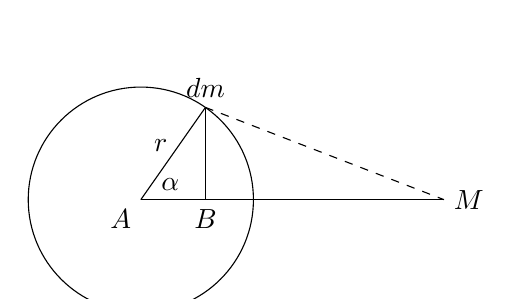
\begin{tikzpicture}[scale=1.1]
  \coordinate (A) at (0,0);
  \coordinate (dm) at (0.746,1.065);
  \coordinate (B) at (0.746,0);
  \coordinate (M) at (3.5,0);
  \draw (A) circle (1.3);
  \draw (A) -- (M);
  \draw (A) -- (dm);
  \draw (B) -- (dm);
  \draw[dashed] (dm) -- (M);
  \node[above] at (dm) {$dm$};
  \node[below left] at (A) {$A$};
  \node[below] at (B) {$B$};
  \node[right] at (M) {$M$};
  \node at (0.34,0.17) {$\alpha$};
  \node[left] at (0.42,0.62) {$r$};
\end{tikzpicture}

$AM = a$;\quad $AB = r\cos\alpha$.
\end{center}

If one assumes a corporeal point, a material element $dm$, which
attracts $M$, and this $dm$ determined by the radius $r$, by the angle
$\alpha$, and by an angle $\Theta$ which a fixed plane forms, for example,
with the plane of the paper; if one further assumes $dm = pdw$, $p$ being
the density and $w$ the volume, so that $dw$ is proved to be
$= r^{2}\sin\Theta\,dr\,d\Theta\,d\alpha$, and the whole
attraction of the point, resolved along the direction toward the centre,
\[
= \frac{kdm\,(a - r\cos\alpha)}{(r^{2} + a^{2} - 2ra\cos\alpha)^{\frac{3}{2}}}
\]
then one can by integration determine the attraction which the whole
mass of the sphere exerts upon $M$,
\[
= k\int \frac{dm\,(a - r\cos\alpha)}
  {(r^{2} + a^{2} - 2ra\cos\alpha)^{\frac{3}{2}}};
\]
but $dm = pdw$, thus one has
\[
kp\int \frac{dw\,(a - r\cos\alpha)}
  {(r^{2} + a^{2} - 2ra\cdot\cos\alpha)^{\frac{3}{2}}}
= kp\int \frac{r^{2}\sin\Theta\,dr\,d\Theta\,d\alpha\,(a - r\cos\alpha)}
  {(r^{2} + a^{2} - 2ra\cos\alpha)^{\frac{3}{2}}}.
\]
But to integrate once with respect to mass is the same as to
integrate 3 times with respect to the variables by which the volume is
expressed. Thus one integrates first with respect to $\Theta$, the angle
which arises as
% ---- printed p.84 (PDF 89) ----
$dm$ is turned in a circle about $AM$ (the limits are $0^{\circ}$ and
$360^{\circ}$, $\int_{0}^{2\pi}$); next one integrates with respect to
$\alpha$ (the limits are $0^{\circ}$ and $180^{\circ}$,
$\int_{0}^{\pi}$, for, when the semicircle moves about its diameter,
the spherical shell arises); finally one must, in order to obtain the infinitely
many spherical shells, integrate with respect to $r$, $\int_{0}^{r}$.

Thus one has, for the force with which the whole mass $m$ attracts $M$,
\[
kp\iiint \frac{r^{2}\sin\Theta\,dr\,d\Theta\,d\alpha\,(a - r\cos\alpha)}
  {(r^{2} + a^{2} - 2ra\cos\alpha)^{\frac{3}{2}}};
\]
and herein a further proof that the infinite, at all points in the
analysis, joins together with the finite, that the infinite is thus
after all finite, and the finite infinite.

\end{document}
